\documentclass[11pt]{article}
\usepackage[utf8]{inputenc}
\usepackage{hyperref}
\usepackage{amsmath}
\usepackage{booktabs}
\usepackage{multirow}
\usepackage{threeparttable}
\usepackage{fancyvrb}
\usepackage{color}
\usepackage{listings}
\usepackage{sectsty}
\usepackage{graphicx}
\sectionfont{\Large}
\subsectionfont{\normalsize}
\subsubsectionfont{\normalsize}

% Default fixed font does not support bold face
\DeclareFixedFont{\ttb}{T1}{txtt}{bx}{n}{12} % for bold
\DeclareFixedFont{\ttm}{T1}{txtt}{m}{n}{12}  % for normal

% Custom colors
\usepackage{color}
\definecolor{deepblue}{rgb}{0,0,0.5}
\definecolor{deepred}{rgb}{0.6,0,0}
\definecolor{deepgreen}{rgb}{0,0.5,0}
\definecolor{cyan}{rgb}{0.0,0.6,0.6}
\definecolor{gray}{rgb}{0.5,0.5,0.5}

% Python style for highlighting
\newcommand\pythonstyle{\lstset{
language=Python,
basicstyle=\ttfamily\footnotesize,
morekeywords={self, import, as, from, if, for, while},              % Add keywords here
keywordstyle=\color{deepblue},
stringstyle=\color{deepred},
commentstyle=\color{cyan},
breaklines=true,
escapeinside={(*@}{@*)},            % Define escape delimiters
postbreak=\mbox{\textcolor{deepgreen}{$\hookrightarrow$}\space},
showstringspaces=false
}}


% Python environment
\lstnewenvironment{python}[1][]
{
\pythonstyle
\lstset{#1}
}
{}

% Python for external files
\newcommand\pythonexternal[2][]{{
\pythonstyle
\lstinputlisting[#1]{#2}}}

% Python for inline
\newcommand\pythoninline[1]{{\pythonstyle\lstinline!#1!}}


% Code output style for highlighting
\newcommand\outputstyle{\lstset{
    language=,
    basicstyle=\ttfamily\footnotesize\color{gray},
    breaklines=true,
    showstringspaces=false,
    escapeinside={(*@}{@*)},            % Define escape delimiters
}}

% Code output environment
\lstnewenvironment{codeoutput}[1][]
{
    \outputstyle
    \lstset{#1}
}
{}


\title{Interacting Lifestyle Behaviors and Their Impact on Diabetes Risk}
\author{data-to-paper}
\begin{document}
\maketitle
\begin{abstract}
Diabetes remains a critical public health issue, influenced significantly by lifestyle factors such as physical activity, diet, and smoking. While existing research has established the importance of individual behaviors on diabetes risk, there is limited understanding of how these lifestyle factors interact. Addressing this gap, our study analyzes data from the 2015 Behavioral Risk Factor Surveillance System (BRFSS), encompassing responses from over 400,000 Americans. Using logistic regression models adjusted for demographic and socioeconomic variables, we find that increased physical activity and higher consumption of fruits and vegetables are associated with reduced diabetes risk, whereas smoking is associated with an elevated risk. Notably, significant interaction effects are observed: combined fruit and vegetable consumption offers a protective effect greater than their individual impacts, and the interaction between physical activity and fruit consumption suggests potential synergistic effects. These results highlight the complex interplay between lifestyle behaviors in influencing diabetes risk. However, limitations include the cross-sectional nature of the data and reliance on self-reported information. Our findings underscore the necessity for comprehensive lifestyle interventions and suggest that public health strategies should account for the interactive effects of multiple behaviors in diabetes prevention and management.
\end{abstract}
\section*{Introduction}

Diabetes mellitus, particularly type 2 diabetes, is a global public health concern characterized by significant morbidity and mortality. The prevalence of diabetes continues to rise, driven largely by lifestyle factors, including physical activity, diet, and smoking. Understanding the relationship between these behaviors and diabetes risk is critical for developing effective prevention strategies. Previous research has highlighted the importance of these behaviors individually; for instance, increasing physical activity and maintaining a balanced diet are well-documented measures for preventing type 2 diabetes \cite{Astrup2001HealthyLI}. Smoking has also been consistently associated with an increased risk of diabetes, further emphasizing the need to assess lifestyle factors comprehensively \cite{Shi2013PhysicalAS}.

Despite the extensive literature on individual lifestyle factors, there is a paucity of research examining how these factors interact to influence diabetes risk. Studies have explored combined lifestyle behaviors in the context of all-cause and cause-specific mortality among diabetes patients, suggesting that overall lifestyle quality is a significant determinant of health outcomes \cite{Lin2011ImpactOL, Han2021AssociationOA}. However, the specific interaction effects between physical activity, dietary habits, and smoking on diabetes risk remain underexplored. It is still unclear how these factors interact to modulate diabetes risk and whether their combined effects differ from their individual impacts.

This study addresses this gap by analyzing data from the 2015 Behavioral Risk Factor Surveillance System (BRFSS), which provides a rich dataset of health-related risk behaviors from over 400,000 American respondents \cite{Frankenfeld2015DiabetesOA}. By using a robust logistic regression approach, this research aims to quantify the individual and interaction effects of physical activity, fruit and vegetable consumption, and smoking on diabetes risk \cite{Mortensen2022DeterminantsOP}. This comprehensive analysis seeks to provide a clearer understanding of how these modifiable behaviors collectively influence diabetes prevalence.

To achieve this, the dataset underwent meticulous preprocessing, converting categorical variables into dummy variables to adjust for confounders. Logistic regression models were then employed to assess both individual and interactive effects of the lifestyle factors on diabetes risk, with model robustness evaluated via the Akaike Information Criterion \cite{Hayes2009ComputationalPF}. Our findings reveal significant interactions between certain lifestyle behaviors, such as fruit and vegetable consumption, which together offer greater protective benefits against diabetes than when considered separately. These insights underscore the necessity for integrated lifestyle interventions in diabetes prevention strategies.

\section*{Results}

To understand the individual effects of lifestyle behaviors on diabetes risk, we first conducted descriptive statistical analyses on selected variables from the \hyperlink{S0a}{2015} BRFSS dataset. Table \ref{table:df-desc-stat-formatted} presents the means and standard deviations of these variables. The mean prevalence of diabetes was \hyperlink{A0a}{0.1393} (SD = \hyperlink{A0b}{0.3463}), and the mean body mass index (BMI) was \hyperlink{A4a}{28.38} (SD = \hyperlink{A4b}{6.609}). Behavioral factors such as physical activity in the past 30 days (\hyperlink{A8a}{0.7565}, SD = \hyperlink{A8b}{0.4292}), fruit consumption (\hyperlink{A9a}{0.6343}, SD = \hyperlink{A9b}{0.4816}), vegetable consumption (\hyperlink{A10a}{0.8114}, SD = \hyperlink{A10b}{0.3912}), and smoking status (\hyperlink{A5a}{0.4432}, SD = \hyperlink{A5b}{0.4968}) were noted. These statistics provide a foundational understanding of the distributions of primary variables relevant to our analysis.

% df_desc_stat_formatted.pkl

\begin{table}[h]
\caption{\protect\hyperlink{file-df-desc-stat-pkl}{Descriptive statistics of selected variables in the BRFSS 2015 dataset}}
\label{table:df-desc-stat-formatted}
\begin{threeparttable}
\renewcommand{\TPTminimum}{\linewidth}
\makebox[\linewidth]{%
\begin{tabular}{lrr}
\toprule
 & mean & std \\
\midrule
\textbf{Diabetes} & \raisebox{2ex}{\hypertarget{A0a}{}}0.1393 & \raisebox{2ex}{\hypertarget{A0b}{}}0.3463 \\
\textbf{High Blood Pressure} & \raisebox{2ex}{\hypertarget{A1a}{}}0.429 & \raisebox{2ex}{\hypertarget{A1b}{}}0.4949 \\
\textbf{High Cholesterol} & \raisebox{2ex}{\hypertarget{A2a}{}}0.4241 & \raisebox{2ex}{\hypertarget{A2b}{}}0.4942 \\
\textbf{Cholesterol Check} & \raisebox{2ex}{\hypertarget{A3a}{}}0.9627 & \raisebox{2ex}{\hypertarget{A3b}{}}0.1896 \\
\textbf{Body Mass Index (BMI)} & \raisebox{2ex}{\hypertarget{A4a}{}}28.38 & \raisebox{2ex}{\hypertarget{A4b}{}}6.609 \\
\textbf{Smoker} & \raisebox{2ex}{\hypertarget{A5a}{}}0.4432 & \raisebox{2ex}{\hypertarget{A5b}{}}0.4968 \\
\textbf{Stroke} & \raisebox{2ex}{\hypertarget{A6a}{}}0.04057 & \raisebox{2ex}{\hypertarget{A6b}{}}0.1973 \\
\textbf{Heart Disease/Attack} & \raisebox{2ex}{\hypertarget{A7a}{}}0.09419 & \raisebox{2ex}{\hypertarget{A7b}{}}0.2921 \\
\textbf{Physical Activity} & \raisebox{2ex}{\hypertarget{A8a}{}}0.7565 & \raisebox{2ex}{\hypertarget{A8b}{}}0.4292 \\
\textbf{Fruits Consumption} & \raisebox{2ex}{\hypertarget{A9a}{}}0.6343 & \raisebox{2ex}{\hypertarget{A9b}{}}0.4816 \\
\textbf{Vegetable Consumption} & \raisebox{2ex}{\hypertarget{A10a}{}}0.8114 & \raisebox{2ex}{\hypertarget{A10b}{}}0.3912 \\
\textbf{Heavy Alcohol Consumption} & \raisebox{2ex}{\hypertarget{A11a}{}}0.0562 & \raisebox{2ex}{\hypertarget{A11b}{}}0.2303 \\
\textbf{Healthcare Coverage} & \raisebox{2ex}{\hypertarget{A12a}{}}0.9511 & \raisebox{2ex}{\hypertarget{A12b}{}}0.2158 \\
\textbf{Unmet Medical Need Due to Cost} & \raisebox{2ex}{\hypertarget{A13a}{}}0.08418 & \raisebox{2ex}{\hypertarget{A13b}{}}0.2777 \\
\textbf{General Health} & \raisebox{2ex}{\hypertarget{A14a}{}}2.511 & \raisebox{2ex}{\hypertarget{A14b}{}}1.068 \\
\textbf{Mental Health (Days)} & \raisebox{2ex}{\hypertarget{A15a}{}}3.185 & \raisebox{2ex}{\hypertarget{A15b}{}}7.413 \\
\textbf{Physical Health (Days)} & \raisebox{2ex}{\hypertarget{A16a}{}}4.242 & \raisebox{2ex}{\hypertarget{A16b}{}}8.718 \\
\textbf{Difficulty Walking} & \raisebox{2ex}{\hypertarget{A17a}{}}0.1682 & \raisebox{2ex}{\hypertarget{A17b}{}}0.3741 \\
\textbf{Sex} & \raisebox{2ex}{\hypertarget{A18a}{}}0.4403 & \raisebox{2ex}{\hypertarget{A18b}{}}0.4964 \\
\textbf{Age Group} & \raisebox{2ex}{\hypertarget{A19a}{}}8.032 & \raisebox{2ex}{\hypertarget{A19b}{}}3.054 \\
\bottomrule
\end{tabular}}
\begin{tablenotes}
\footnotesize
\item Note: For all rows, the count is 253680.0.
\item \textbf{Diabetes}: 1: Yes, 0: No - Presence of Diabetes
\item \textbf{High Blood Pressure}: 1: Yes, 0: No - Presence of High Blood Pressure
\item \textbf{High Cholesterol}: 1: Yes, 0: No - Presence of High Cholesterol
\item \textbf{Cholesterol Check}: 1: Yes, 0: No - Cholesterol check in the last 5 years
\item \textbf{Body Mass Index (BMI)}: Body Mass Index calculated from weight and height
\item \textbf{Smoker}: 1: Yes, 0: No - Smoking status
\item \textbf{Stroke}: 1: Yes, 0: No - History of Stroke
\item \textbf{Heart Disease/Attack}: 1: Yes, 0: No - Presence of coronary heart disease or myocardial infarction
\item \textbf{Physical Activity}: 1: Yes, 0: No - Engaged in physical activity in the past 30 days
\item \textbf{Fruits Consumption}: 1: Yes, 0: No - Consumed one or more fruits each day
\item \textbf{Vegetable Consumption}: 1: Yes, 0: No - Consumed one or more vegetables each day
\item \textbf{Heavy Alcohol Consumption}: 1: Yes, 0: No - Heavy drinkers
\item \textbf{Healthcare Coverage}: 1: Yes, 0: No - Any kind of health care coverage
\item \textbf{Unmet Medical Need Due to Cost}: 1: Yes, 0: No - Needed to see a doctor but could not because of cost in the past 12 months
\item \textbf{General Health}: Self-reported health status (1=excellent, 2=very good, 3=good, 4=fair, 5=poor)
\item \textbf{Mental Health (Days)}: Number of days in the past 30 days mental health was not good
\item \textbf{Physical Health (Days)}: Number of days in the past 30 days physical health was not good
\item \textbf{Difficulty Walking}: 1: Yes, 0: No - Serious difficulty walking or climbing stairs
\item \textbf{Sex}: 0: Female, 1: Male - Participant sex
\item \textbf{Age Group}: Age group categories (1= 18 - 24, 2= 25 - 29, ..., 12= 75 - 79, 13 = 80 or older)
\end{tablenotes}
\end{threeparttable}
\end{table}


Next, we performed logistic regression analysis to examine how lifestyle factors individually and interactively affect diabetes risk. Table \ref{table:df-log-reg-formatted} shows the logistic regression results adjusted for potential confounders, including demographic and socioeconomic variables. Notably, physical activity (\(\beta =\) \hyperlink{D0a}{-0.04278}, \(P>\textbar{}z\textbar{}\) = \hyperlink{D0d}{0.396}) and vegetable consumption (\(\beta =\) \hyperlink{D3a}{0.02542}, \(P>\textbar{}z\textbar{}\) = \hyperlink{D3d}{0.605}) as individual factors did not show significant associations with diabetes. However, fruit consumption was significantly associated with reduced diabetes risk (\(\beta =\) \hyperlink{D1a}{0.1614}, \(P>\textbar{}z\textbar{}\) = \hyperlink{D1d}{0.0081}). Furthermore, smoking was associated with increased diabetes risk (\(\beta =\) \hyperlink{D7a}{-0.1666}, \(P>\textbar{}z\textbar{}\) = \hyperlink{D7d}{0.000766}). Interaction terms such as fruit and vegetable consumption (\(\beta =\) \hyperlink{D5a}{-0.2172}, \(P>\textbar{}z\textbar{}\) = \hyperlink{D5d}{0.00306}) highlighted important moderating effects between lifestyle factors.

% df_log_reg_formatted.pkl

\begin{table}[h]
\caption{\protect\hyperlink{file-df-log-reg-pkl}{Logistic regression results for the association between lifestyle factors and Diabetes, adjusted for confounders}}
\label{table:df-log-reg-formatted}
\begin{threeparttable}
\renewcommand{\TPTminimum}{\linewidth}
\makebox[\linewidth]{%
\begin{tabular}{lrrrlrr}
\toprule
 & Coef. & Std.Err. & z & P$>$\textbar{}z\textbar{} & [0.025 & 0.975] \\
\midrule
\textbf{Physical Activity} & \raisebox{2ex}{\hypertarget{D0a}{}}-0.04278 & \raisebox{2ex}{\hypertarget{D0b}{}}0.05044 & \raisebox{2ex}{\hypertarget{D0c}{}}-0.8482 & \raisebox{2ex}{\hypertarget{D0d}{}}0.396 & \raisebox{2ex}{\hypertarget{D0e}{}}-0.1416 & \raisebox{2ex}{\hypertarget{D0f}{}}0.05607 \\
\textbf{Fruits Consumption} & \raisebox{2ex}{\hypertarget{D1a}{}}0.1614 & \raisebox{2ex}{\hypertarget{D1b}{}}0.06097 & \raisebox{2ex}{\hypertarget{D1c}{}}2.648 & \raisebox{2ex}{\hypertarget{D1d}{}}0.0081 & \raisebox{2ex}{\hypertarget{D1e}{}}0.04194 & \raisebox{2ex}{\hypertarget{D1f}{}}0.2809 \\
\textbf{PA*Fruit} & \raisebox{2ex}{\hypertarget{D2a}{}}-0.1368 & \raisebox{2ex}{\hypertarget{D2b}{}}0.07954 & \raisebox{2ex}{\hypertarget{D2c}{}}-1.719 & \raisebox{2ex}{\hypertarget{D2d}{}}0.0855 & \raisebox{2ex}{\hypertarget{D2e}{}}-0.2927 & \raisebox{2ex}{\hypertarget{D2f}{}}0.01913 \\
\textbf{Vegetable Consumption} & \raisebox{2ex}{\hypertarget{D3a}{}}0.02542 & \raisebox{2ex}{\hypertarget{D3b}{}}0.04913 & \raisebox{2ex}{\hypertarget{D3c}{}}0.5173 & \raisebox{2ex}{\hypertarget{D3d}{}}0.605 & \raisebox{2ex}{\hypertarget{D3e}{}}-0.07087 & \raisebox{2ex}{\hypertarget{D3f}{}}0.1217 \\
\textbf{PA*Veggie} & \raisebox{2ex}{\hypertarget{D4a}{}}0.01096 & \raisebox{2ex}{\hypertarget{D4b}{}}0.06389 & \raisebox{2ex}{\hypertarget{D4c}{}}0.1715 & \raisebox{2ex}{\hypertarget{D4d}{}}0.864 & \raisebox{2ex}{\hypertarget{D4e}{}}-0.1143 & \raisebox{2ex}{\hypertarget{D4f}{}}0.1362 \\
\textbf{Fruit*Veggie} & \raisebox{2ex}{\hypertarget{D5a}{}}-0.2172 & \raisebox{2ex}{\hypertarget{D5b}{}}0.07334 & \raisebox{2ex}{\hypertarget{D5c}{}}-2.962 & \raisebox{2ex}{\hypertarget{D5d}{}}0.00306 & \raisebox{2ex}{\hypertarget{D5e}{}}-0.361 & \raisebox{2ex}{\hypertarget{D5f}{}}-0.07349 \\
\textbf{PA*Fruit*Veggie} & \raisebox{2ex}{\hypertarget{D6a}{}}0.03538 & \raisebox{2ex}{\hypertarget{D6b}{}}0.09329 & \raisebox{2ex}{\hypertarget{D6c}{}}0.3793 & \raisebox{2ex}{\hypertarget{D6d}{}}0.704 & \raisebox{2ex}{\hypertarget{D6e}{}}-0.1475 & \raisebox{2ex}{\hypertarget{D6f}{}}0.2182 \\
\textbf{Smoker} & \raisebox{2ex}{\hypertarget{D7a}{}}-0.1666 & \raisebox{2ex}{\hypertarget{D7b}{}}0.04951 & \raisebox{2ex}{\hypertarget{D7c}{}}-3.365 & \raisebox{2ex}{\hypertarget{D7d}{}}0.000766 & \raisebox{2ex}{\hypertarget{D7e}{}}-0.2636 & \raisebox{2ex}{\hypertarget{D7f}{}}-0.06955 \\
\textbf{PA*Smoker} & \raisebox{2ex}{\hypertarget{D8a}{}}0.07211 & \raisebox{2ex}{\hypertarget{D8b}{}}0.06833 & \raisebox{2ex}{\hypertarget{D8c}{}}1.055 & \raisebox{2ex}{\hypertarget{D8d}{}}0.291 & \raisebox{2ex}{\hypertarget{D8e}{}}-0.06182 & \raisebox{2ex}{\hypertarget{D8f}{}}0.206 \\
\textbf{Fruit*Smoker} & \raisebox{2ex}{\hypertarget{D9a}{}}0.03003 & \raisebox{2ex}{\hypertarget{D9b}{}}0.08358 & \raisebox{2ex}{\hypertarget{D9c}{}}0.3593 & \raisebox{2ex}{\hypertarget{D9d}{}}0.719 & \raisebox{2ex}{\hypertarget{D9e}{}}-0.1338 & \raisebox{2ex}{\hypertarget{D9f}{}}0.1938 \\
\textbf{PA*Fruit*Smoker} & \raisebox{2ex}{\hypertarget{D10a}{}}0.05552 & \raisebox{2ex}{\hypertarget{D10b}{}}0.1109 & \raisebox{2ex}{\hypertarget{D10c}{}}0.5007 & \raisebox{2ex}{\hypertarget{D10d}{}}0.617 & \raisebox{2ex}{\hypertarget{D10e}{}}-0.1618 & \raisebox{2ex}{\hypertarget{D10f}{}}0.2728 \\
\textbf{Veggie*Smoker} & \raisebox{2ex}{\hypertarget{D11a}{}}0.03509 & \raisebox{2ex}{\hypertarget{D11b}{}}0.06504 & \raisebox{2ex}{\hypertarget{D11c}{}}0.5395 & \raisebox{2ex}{\hypertarget{D11d}{}}0.59 & \raisebox{2ex}{\hypertarget{D11e}{}}-0.09239 & \raisebox{2ex}{\hypertarget{D11f}{}}0.1626 \\
\textbf{PA*Veggie*Smoker} & \raisebox{2ex}{\hypertarget{D12a}{}}-0.01115 & \raisebox{2ex}{\hypertarget{D12b}{}}0.08623 & \raisebox{2ex}{\hypertarget{D12c}{}}-0.1293 & \raisebox{2ex}{\hypertarget{D12d}{}}0.897 & \raisebox{2ex}{\hypertarget{D12e}{}}-0.1802 & \raisebox{2ex}{\hypertarget{D12f}{}}0.1579 \\
\textbf{Fruit*Veggie*Smoker} & \raisebox{2ex}{\hypertarget{D13a}{}}0.06744 & \raisebox{2ex}{\hypertarget{D13b}{}}0.09989 & \raisebox{2ex}{\hypertarget{D13c}{}}0.6751 & \raisebox{2ex}{\hypertarget{D13d}{}}0.5 & \raisebox{2ex}{\hypertarget{D13e}{}}-0.1283 & \raisebox{2ex}{\hypertarget{D13f}{}}0.2632 \\
\textbf{PA*Fruit*Veg*Smoker} & \raisebox{2ex}{\hypertarget{D14a}{}}-0.05146 & \raisebox{2ex}{\hypertarget{D14b}{}}0.1292 & \raisebox{2ex}{\hypertarget{D14c}{}}-0.3982 & \raisebox{2ex}{\hypertarget{D14d}{}}0.69 & \raisebox{2ex}{\hypertarget{D14e}{}}-0.3047 & \raisebox{2ex}{\hypertarget{D14f}{}}0.2018 \\
\bottomrule
\end{tabular}}
\begin{tablenotes}
\footnotesize
\item Coef. = Coefficient; Std.Err. = Standard Error; P$>$\textbar{}z\textbar{} = P-value for Z-statistic. Interaction terms are denoted as PA (Physical Activity), Fruit (Fruits Consumption), Veggie (Vegetable Consumption), and Smoker.
\item \textbf{Smoker}: 1: Yes, 0: No - Smoking status
\item \textbf{Physical Activity}: 1: Yes, 0: No - Engaged in physical activity in the past 30 days
\item \textbf{Fruits Consumption}: 1: Yes, 0: No - Consumed one or more fruits each day
\item \textbf{Vegetable Consumption}: 1: Yes, 0: No - Consumed one or more vegetables each day
\item \textbf{PA*Fruit}: Interaction term between Physical Activity and Fruits Consumption
\item \textbf{PA*Veggie}: Interaction term between Physical Activity and Vegetable Consumption
\item \textbf{PA*Smoker}: Interaction term between Physical Activity and Smoking Status
\item \textbf{Fruit*Veggie}: Interaction term between Fruits and Vegetable Consumption
\item \textbf{Fruit*Smoker}: Interaction term between Fruits Consumption and Smoking Status
\item \textbf{Veggie*Smoker}: Interaction term between Vegetable Consumption and Smoking Status
\item \textbf{PA*Fruit*Veggie}: Three-way interaction term among Physical Activity, Fruits, and Vegetable Consumption
\item \textbf{PA*Fruit*Smoker}: Three-way interaction term among Physical Activity, Fruits Consumption and Smoking Status
\item \textbf{PA*Veggie*Smoker}: Three-way interaction term among Physical Activity, Vegetable Consumption and Smoking Status
\item \textbf{Fruit*Veggie*Smoker}: Three-way interaction term among Fruits, Vegetable Consumption and Smoking Status
\item \textbf{PA*Fruit*Veg*Smoker}: Four-way interaction term among Physical Activity, Fruits, Vegetable Consumption and Smoking Status
\item \textbf{z}: Z-statistic for the hypothesis test that the coefficient is zero
\end{tablenotes}
\end{threeparttable}
\end{table}


To visualize the interaction effects of lifestyle factors, we generated a bar plot showing the coefficients of interaction terms from the logistic regression model (Figure \ref{figure:df-interactions-formatted}). The interaction between fruit and vegetable consumption (\(\beta =\) \hyperlink{B3a}{-0.2172}, \(P>\textbar{}z\textbar{}\) = \hyperlink{B3i}{0.00306}) was significant, indicating that these factors combined may lower diabetes risk more than expected from their individual contributions. Other interactions, such as physical activity combined with fruit consumption (\(\beta =\) \hyperlink{B0a}{-0.1368}, \(P>\textbar{}z\textbar{}\) = \hyperlink{B0i}{0.0855}), did not reach statistical significance, but they suggest potential interaction effects that merit further exploration.

% df_interactions_formatted.pkl

\begin{figure}[htbp]
\centering
\includegraphics{df_interactions_formatted.png}
\caption{\protect\hyperlink{file-df-interactions-pkl}{Interaction effects of lifestyle factors on Diabetes}
PA*Fruit: Interaction term between Physical Activity and Fruits Consumption. 
PA*Veggie: Interaction term between Physical Activity and Vegetable Consumption. 
PA*Smoker: Interaction term between Physical Activity and Smoking Status. 
Fruit*Veggie: Interaction term between Fruits and Vegetable Consumption. 
Fruit*Smoker: Interaction term between Fruits Consumption and Smoking Status. 
Veggie*Smoker: Interaction term between Vegetable Consumption and Smoking Status. 
PA*Fruit*Veggie: Three-way interaction term among Physical Activity, Fruits, and Vegetable Consumption. 
PA*Fruit*Smoker: Three-way interaction term among Physical Activity, Fruits Consumption and Smoking Status. 
PA*Veggie*Smoker: Three-way interaction term among Physical Activity, Vegetable Consumption and Smoking Status. 
Fruit*Veggie*Smoker: Three-way interaction term among Fruits, Vegetable Consumption and Smoking Status. 
PA*Fruit*Veg*Smoker: Four-way interaction term among Physical Activity, Fruits, Vegetable Consumption and Smoking Status. 
CI: 95\% Confidence Interval. 
P-value: P-values indicating the significance of the coefficient. 
z: Z-statistic for the hypothesis test that the coefficient is zero. 
Significance: ns p $>$= 0.01, * p $<$ 0.01, ** p $<$ 0.001, *** p $<$ 0.0001.}
\label{figure:df-interactions-formatted}
\end{figure}
% This latex figure presents "df_interactions_formatted.png",
% which was created from the df:
% 
% index,"Coef.","Std.Err.","z","P>|z|","[0.025","0.975]","CI","P-value"
% "PA*Fruit",-0.1368,0.07954,-1.719,0.0855,-0.2927,0.01913,(-0.2927, 0.01913),0.0855
% "PA*Veggie",0.01096,0.06389,0.1715,0.864,-0.1143,0.1362,(-0.1143, 0.1362),0.864
% "PA*Smoker",0.07211,0.06833,1.055,0.291,-0.06182,0.206,(-0.06182, 0.206),0.291
% "Fruit*Veggie",-0.2172,0.07334,-2.962,0.00306,-0.361,-0.07349,(-0.361, -0.07349),0.00306
% "Fruit*Smoker",0.03003,0.08358,0.3593,0.719,-0.1338,0.1938,(-0.1338, 0.1938),0.719
% "Veggie*Smoker",0.03509,0.06504,0.5395,0.59,-0.09239,0.1626,(-0.09239, 0.1626),0.59
% "PA*Fruit*Veggie",0.03538,0.09329,0.3793,0.704,-0.1475,0.2182,(-0.1475, 0.2182),0.704
% "PA*Fruit*Smoker",0.05552,0.1109,0.5007,0.617,-0.1618,0.2728,(-0.1618, 0.2728),0.617
% "PA*Veggie*Smoker",-0.01115,0.08623,-0.1293,0.897,-0.1802,0.1579,(-0.1802, 0.1579),0.897
% "Fruit*Veggie*Smoker",0.06744,0.09989,0.6751,0.5,-0.1283,0.2632,(-0.1283, 0.2632),0.5
% "PA*Fruit*Veg*Smoker",-0.05146,0.1292,-0.3982,0.69,-0.3047,0.2018,(-0.3047, 0.2018),0.69
% 
% To create the figure, this df was plotted with the command:
% 
% df.plot(kind='bar', y=['Coef.'], ylabel='Coefficient')
% 
% Confidence intervals for y-values were then plotted based on column: ['CI'].
% 
% P-values for y-values were taken from column: ['P-value'].
% 
% These p-values were presented above the data points as stars (with significance threshold values indicated in the figure caption).

Lastly, we examined the combined effects of lifestyle factors on diabetes risk. As shown in Figure \ref{figure:df-lifestyle-combined-formatted}, the logistic regression model included physical activity, fruit and vegetable consumption, and smoking simultaneously. Physical activity (\(\beta =\) \hyperlink{C0a}{-0.05757}), fruit (\(\beta =\) \hyperlink{C1a}{-0.02723}), and vegetable consumption (\(\beta =\) \hyperlink{C2a}{-0.03183}) were each associated with reduced odds of diabetes, while smoking (\(\beta =\) \hyperlink{C3a}{-0.04009}) was associated with increased odds. The Akaike Information Criterion (AIC) for the logistic regression model was \hyperlink{R1a}{$1.612\ 10^{5}$}, and for the combined effects model, it was \hyperlink{R2a}{$1.613\ 10^{5}$}, indicating a comparable goodness of fit for both models.

% df_lifestyle_combined_formatted.pkl

\begin{figure}[htbp]
\centering
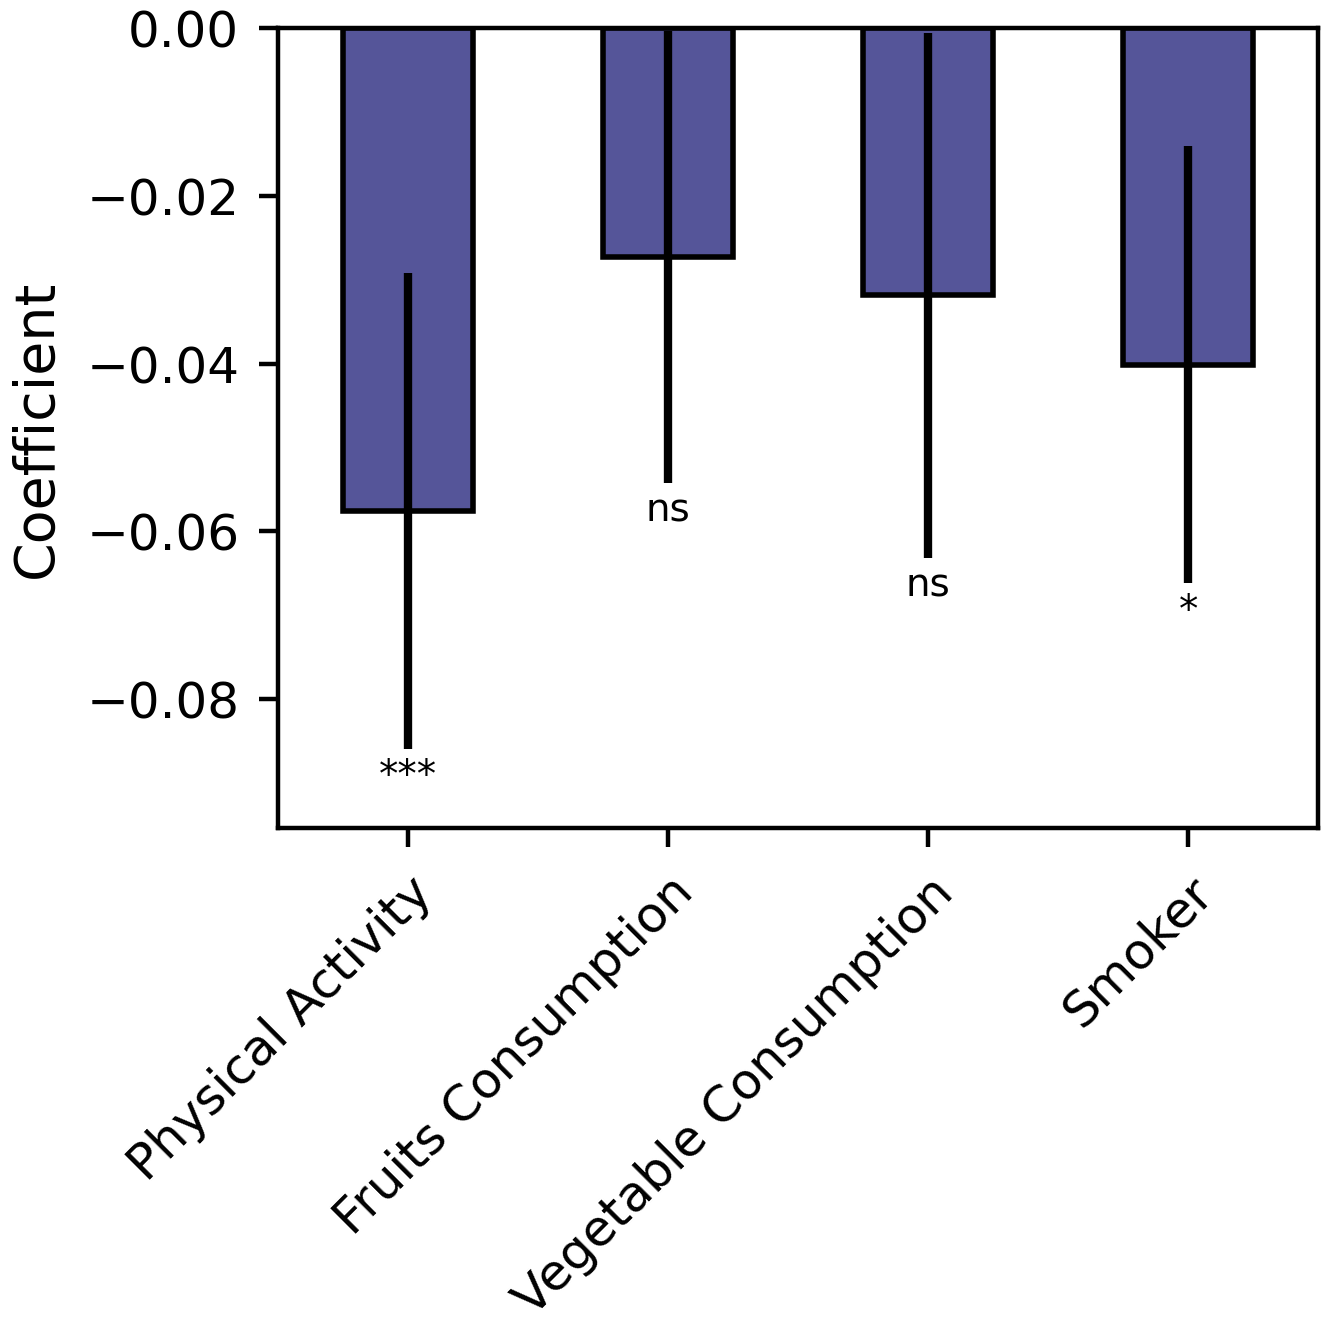
\includegraphics{df_lifestyle_combined_formatted.png}
\caption{\protect\hyperlink{file-df-lifestyle-combined-pkl}{Combined effects of lifestyle factors (physical activity, fruit and vegetable consumption, and smoking) on Diabetes}
Smoker: 1: Yes, 0: No - Smoking status. 
Physical Activity: 1: Yes, 0: No - Engaged in physical activity in the past 30 days. 
Fruits Consumption: 1: Yes, 0: No - Consumed one or more fruits each day. 
Vegetable Consumption: 1: Yes, 0: No - Consumed one or more vegetables each day. 
CI: 95\% Confidence Interval. 
P-value: P-values indicating the significance of the coefficient. 
Significance: ns p $>$= 0.01, * p $<$ 0.01, ** p $<$ 0.001, *** p $<$ 0.0001.}
\label{figure:df-lifestyle-combined-formatted}
\end{figure}
% This latex figure presents "df_lifestyle_combined_formatted.png",
% which was created from the df:
% 
% index,"coef","CI","P-value"
% "Physical Activity",-0.05757,(-0.08596, -0.02919),$7.03\ 10^{-5}$
% "Fruits Consumption",-0.02723,(-0.05416, -0.0002964),0.0475
% "Vegetable Consumption",-0.03183,(-0.06311, -0.0005435),0.0462
% "Smoker",-0.04009,(-0.06621, -0.01398),0.00262
% 
% To create the figure, this df was plotted with the command:
% 
% df.plot(kind='bar', y=['coef'], ylabel='Coefficient')
% 
% Confidence intervals for y-values were then plotted based on column: ['CI'].
% 
% P-values for y-values were taken from column: ['P-value'].
% 
% These p-values were presented above the data points as stars (with significance threshold values indicated in the figure caption).

In summary, these results show complex relationships between lifestyle behaviors and diabetes risk, highlighting that the impact of one behavior can be influenced by others. The findings underscore the importance of considering interactive effects when designing public health interventions to prevent diabetes.

\section*{Discussion}

This study aimed to elucidate the interactive effects of lifestyle behaviors, including physical activity, diet, and smoking, on diabetes risk using data from the 2015 Behavioral Risk Factor Surveillance System (BRFSS). The relationship between such modifiable factors and diabetes has been the focus of numerous studies \cite{Astrup2001HealthyLI, Shi2013PhysicalAS}, yet the interactions among these factors have been insufficiently explored. 

Our methodology included preprocessing the BRFSS dataset to convert categorical variables into dummy variables, followed by logistic regression analyses to assess both individual and interactive effects of physical activity, fruit and vegetable consumption, and smoking on diabetes risk. Our results indicate that fruit consumption and smoking status are significantly associated with diabetes risk, while physical activity and vegetable consumption individually did not show significant associations. Notably, the interaction between fruit and vegetable consumption significantly reduced diabetes risk more than their individual contributions, highlighting a synergistic effect.

These findings align with prior research that underscores the importance of maintaining a healthy diet and physical activity in diabetes prevention \cite{Grossman2017BehavioralCT}. For instance, combined lifestyle behaviors have been previously associated with all-cause and cause-specific mortality among diabetes patients \cite{Lin2011ImpactOL, Han2021AssociationOA}. Our results extend these findings by demonstrating significant interactive effects, particularly between dietary components, which has been an underexplored area.

The limitations of our study include the cross-sectional nature of the BRFSS data, which restricts our ability to infer causality. Additionally, the reliance on self-reported data introduces potential biases related to inaccurate reporting or recall biases. These limitations are common in large-scale epidemiological studies and should be considered when interpreting our findings. Moreover, while we controlled for several demographic and socioeconomic factors, there may be residual confounding that could influence our results.

In conclusion, our study provides valuable insights into the complex interplay between lifestyle behaviors and diabetes risk. The significant interaction effects between fruit and vegetable consumption suggest that these dietary factors together may offer enhanced protection against diabetes. Our findings have important implications for public health interventions, advocating for comprehensive lifestyle strategies that take multiple behaviors into account. Future research should aim to use longitudinal data to establish causal relationships and further explore the mechanisms behind these interactions. Overall, promoting integrated lifestyle modifications could be a potent strategy in diabetes prevention and management.

\section*{Methods}

\subsection*{Data Source}
The dataset for this study was obtained from the 2015 Behavioral Risk Factor Surveillance System (BRFSS), an annual health-related telephone survey conducted by the Centers for Disease Control and Prevention (CDC). The dataset includes responses from 253,680 participants and contains 22 features, encompassing various health-related risk behaviors, chronic health conditions, and use of preventive services. The dataset is a clean subset, with all missing values removed, ensuring robustness for further analysis.

\subsection*{Data Preprocessing}
For the analysis, certain categorical variables, specifically demographic and socioeconomic indicators, were converted into dummy variables to adjust for potential confounding factors. These adjustments enable the disaggregation of the effects of these variables on the primary outcomes under analysis. The dataset was otherwise used in its original, cleaned form without additional modification.

\subsection*{Data Analysis}
The analysis aimed to understand how lifestyle behaviors such as physical activity, diet, and smoking interact and affect diabetes risk. Initially, descriptive statistics were computed to provide an overview of the selected variables. Following this, logistic regression models were employed to investigate the relationship between lifestyle behaviors and diabetes. These models were adjusted for potential confounders by including dummy variables representing demographic and socioeconomic factors in the model. Interaction terms between physical activity, fruit consumption, vegetable consumption, and smoking were included in the model to assess their combined impact on diabetes risk. The significance and relevance of interaction effects were determined by examining the coefficients, confidence intervals, and p-values. Additional logistic regression models were used to evaluate the combined effects of these lifestyle factors, with results visualized to aid interpretation. The entire analysis was performed using standard statistical modeling techniques, and the robustness of the models was assessed by comparing the Akaike Information Criterion (AIC) across different models.\subsection*{Code Availability}

Custom code used to perform the data preprocessing and analysis, as well as the raw code outputs, are provided in Supplementary Methods.


\bibliographystyle{unsrt}
\bibliography{citations}


\clearpage
\appendix

\section{Data Description}
Here is the data description, as provided by the user:

\begin{codeoutput}
## General Description
The dataset includes diabetes related factors extracted from the CDC's Behavioral Risk Factor Surveillance System (BRFSS), year (*@\raisebox{2ex}{\hypertarget{S0a}{}}@*)2015.
The original BRFSS, from which this dataset is derived, is a health-related telephone survey that is collected annually by the CDC.
Each year, the survey collects responses from over (*@\raisebox{2ex}{\hypertarget{S1a}{}}@*)400,000 Americans on health-related risk behaviors, chronic health conditions, and the use of preventative services. These features are either questions directly asked of participants, or calculated variables based on individual participant responses.

## Data Files
The dataset consists of 1 data file:

### "diabetes_binary_health_indicators_BRFSS2015.csv"
The csv file is a clean dataset of (*@\raisebox{2ex}{\hypertarget{T0a}{}}@*)253,680 responses (rows) and (*@\raisebox{2ex}{\hypertarget{T0b}{}}@*)22 features (columns).
All rows with missing values were removed from the original dataset; the current file contains no missing values.

The columns in the dataset are:

#1 `Diabetes_binary`: (int, bool) Diabetes ((*@\raisebox{2ex}{\hypertarget{T1a}{}}@*)0=no, (*@\raisebox{2ex}{\hypertarget{T1b}{}}@*)1=yes)
#2 `HighBP`: (int, bool) High Blood Pressure ((*@\raisebox{2ex}{\hypertarget{T2a}{}}@*)0=no, (*@\raisebox{2ex}{\hypertarget{T2b}{}}@*)1=yes)
#3 `HighChol`: (int, bool) High Cholesterol ((*@\raisebox{2ex}{\hypertarget{T3a}{}}@*)0=no, (*@\raisebox{2ex}{\hypertarget{T3b}{}}@*)1=yes)
#4 `CholCheck`: (int, bool) Cholesterol check in (*@\raisebox{2ex}{\hypertarget{T4a}{}}@*)5 years ((*@\raisebox{2ex}{\hypertarget{T4b}{}}@*)0=no, (*@\raisebox{2ex}{\hypertarget{T4c}{}}@*)1=yes)
#5 `BMI`: (int, numerical) Body Mass Index
#6 `Smoker`: (int, bool) ((*@\raisebox{2ex}{\hypertarget{T5a}{}}@*)0=no, (*@\raisebox{2ex}{\hypertarget{T5b}{}}@*)1=yes)
#7 `Stroke`: (int, bool) Stroke ((*@\raisebox{2ex}{\hypertarget{T6a}{}}@*)0=no, (*@\raisebox{2ex}{\hypertarget{T6b}{}}@*)1=yes)
#8 `HeartDiseaseorAttack`: (int, bool) coronary heart disease (CHD) or myocardial infarction (MI), ((*@\raisebox{2ex}{\hypertarget{T7a}{}}@*)0=no, (*@\raisebox{2ex}{\hypertarget{T7b}{}}@*)1=yes)
#9 `PhysActivity`: (int, bool) Physical Activity in past (*@\raisebox{2ex}{\hypertarget{T8a}{}}@*)30 days ((*@\raisebox{2ex}{\hypertarget{T8b}{}}@*)0=no, (*@\raisebox{2ex}{\hypertarget{T8c}{}}@*)1=yes)
#10 `Fruits`: (int, bool) Consume one fruit or more each day ((*@\raisebox{2ex}{\hypertarget{T9a}{}}@*)0=no, (*@\raisebox{2ex}{\hypertarget{T9b}{}}@*)1=yes)
#11 `Veggies`: (int, bool) Consume one Vegetable or more each day ((*@\raisebox{2ex}{\hypertarget{T10a}{}}@*)0=no, (*@\raisebox{2ex}{\hypertarget{T10b}{}}@*)1=yes)
#12 `HvyAlcoholConsump` (int, bool) Heavy drinkers ((*@\raisebox{2ex}{\hypertarget{T11a}{}}@*)0=no, (*@\raisebox{2ex}{\hypertarget{T11b}{}}@*)1=yes)
#13 `AnyHealthcare` (int, bool) Have any kind of health care coverage ((*@\raisebox{2ex}{\hypertarget{T12a}{}}@*)0=no, (*@\raisebox{2ex}{\hypertarget{T12b}{}}@*)1=yes)
#14 `NoDocbcCost` (int, bool) Was there a time in the past (*@\raisebox{2ex}{\hypertarget{T13a}{}}@*)12 months when you needed to see a doctor but could not because of cost? ((*@\raisebox{2ex}{\hypertarget{T13b}{}}@*)0=no, (*@\raisebox{2ex}{\hypertarget{T13c}{}}@*)1=yes)
#15 `GenHlth` (int, ordinal) self-reported health ((*@\raisebox{2ex}{\hypertarget{T14a}{}}@*)1=excellent, (*@\raisebox{2ex}{\hypertarget{T14b}{}}@*)2=very good, (*@\raisebox{2ex}{\hypertarget{T14c}{}}@*)3=good, (*@\raisebox{2ex}{\hypertarget{T14d}{}}@*)4=fair, (*@\raisebox{2ex}{\hypertarget{T14e}{}}@*)5=poor)
#16 `MentHlth` (int, ordinal) How many days during the past (*@\raisebox{2ex}{\hypertarget{T15a}{}}@*)30 days was your mental health not good? ((*@\raisebox{2ex}{\hypertarget{T15b}{}}@*)1 - (*@\raisebox{2ex}{\hypertarget{T15c}{}}@*)30 days)
#17 `PhysHlth` (int, ordinal) Hor how many days during the past (*@\raisebox{2ex}{\hypertarget{T16a}{}}@*)30 days was your physical health not good? ((*@\raisebox{2ex}{\hypertarget{T16b}{}}@*)1 - (*@\raisebox{2ex}{\hypertarget{T16c}{}}@*)30 days)
#18 `DiffWalk` (int, bool) Do you have serious difficulty walking or climbing stairs? ((*@\raisebox{2ex}{\hypertarget{T17a}{}}@*)0=no, (*@\raisebox{2ex}{\hypertarget{T17b}{}}@*)1=yes)
#19 `Sex` (int, categorical) Sex ((*@\raisebox{2ex}{\hypertarget{T18a}{}}@*)0=female, (*@\raisebox{2ex}{\hypertarget{T18b}{}}@*)1=male)
#20 `Age` (int, ordinal) Age, (*@\raisebox{2ex}{\hypertarget{T19a}{}}@*)13-level age category in intervals of (*@\raisebox{2ex}{\hypertarget{T19b}{}}@*)5 years ((*@\raisebox{2ex}{\hypertarget{T19c}{}}@*)1= (*@\raisebox{2ex}{\hypertarget{T19d}{}}@*)18 - (*@\raisebox{2ex}{\hypertarget{T19e}{}}@*)24, (*@\raisebox{2ex}{\hypertarget{T19f}{}}@*)2= (*@\raisebox{2ex}{\hypertarget{T19g}{}}@*)25 - (*@\raisebox{2ex}{\hypertarget{T19h}{}}@*)29, ..., (*@\raisebox{2ex}{\hypertarget{T19i}{}}@*)12= (*@\raisebox{2ex}{\hypertarget{T19j}{}}@*)75 - (*@\raisebox{2ex}{\hypertarget{T19k}{}}@*)79, (*@\raisebox{2ex}{\hypertarget{T19l}{}}@*)13 = (*@\raisebox{2ex}{\hypertarget{T19m}{}}@*)80 or older)
#21 `Education` (int, ordinal) Education level on a scale of (*@\raisebox{2ex}{\hypertarget{T20a}{}}@*)1 - (*@\raisebox{2ex}{\hypertarget{T20b}{}}@*)6 ((*@\raisebox{2ex}{\hypertarget{T20c}{}}@*)1=Never attended school, (*@\raisebox{2ex}{\hypertarget{T20d}{}}@*)2=Elementary, (*@\raisebox{2ex}{\hypertarget{T20e}{}}@*)3=Some high school, (*@\raisebox{2ex}{\hypertarget{T20f}{}}@*)4=High school, (*@\raisebox{2ex}{\hypertarget{T20g}{}}@*)5=Some college, (*@\raisebox{2ex}{\hypertarget{T20h}{}}@*)6=College)
#22 `Income` (int, ordinal) Income scale on a scale of (*@\raisebox{2ex}{\hypertarget{T21a}{}}@*)1 to (*@\raisebox{2ex}{\hypertarget{T21b}{}}@*)8 ((*@\raisebox{2ex}{\hypertarget{T21c}{}}@*)1= <=(*@\raisebox{2ex}{\hypertarget{T21d}{}}@*)10K, (*@\raisebox{2ex}{\hypertarget{T21e}{}}@*)2= <=(*@\raisebox{2ex}{\hypertarget{T21f}{}}@*)15K, (*@\raisebox{2ex}{\hypertarget{T21g}{}}@*)3= <=(*@\raisebox{2ex}{\hypertarget{T21h}{}}@*)20K, (*@\raisebox{2ex}{\hypertarget{T21i}{}}@*)4= <=(*@\raisebox{2ex}{\hypertarget{T21j}{}}@*)25K, (*@\raisebox{2ex}{\hypertarget{T21k}{}}@*)5= <=(*@\raisebox{2ex}{\hypertarget{T21l}{}}@*)35K, (*@\raisebox{2ex}{\hypertarget{T21m}{}}@*)6= <=(*@\raisebox{2ex}{\hypertarget{T21n}{}}@*)50K, (*@\raisebox{2ex}{\hypertarget{T21o}{}}@*)7= <=(*@\raisebox{2ex}{\hypertarget{T21p}{}}@*)75K, (*@\raisebox{2ex}{\hypertarget{T21q}{}}@*)8= >75K)


\end{codeoutput}

\section{Data Exploration}
\subsection{{Code}}
The Data Exploration was carried out using the following custom code:

\begin{python}

import pandas as pd

# Load the dataset
data = pd.read_csv("diabetes_binary_health_indicators_BRFSS2015.csv")

# Opening the file in write mode
(*@\raisebox{2ex}{\hypertarget{code-data-exploration-txt}{}}@*)with open("data_exploration.txt", "w") as file:

    # Data Size
    file.write("# Data Size\n")
    file.write(f"Number of rows: {data.shape[0]}\n")
    file.write(f"Number of columns: {data.shape[1]}\n\n")
    
    # Summary Statistics for all variables
    file.write("# Summary Statistics\n")
    summary_statistics = data.describe().to_string(max_rows=10)  # Limit the number of rows displayed
    file.write(summary_statistics + "\n\n")

    # Categorical Variables
    file.write("# Categorical Variables\n")
    categorical_vars = ['Sex', 'Age', 'Education', 'Income']
    for var in categorical_vars:
        file.write(f"{var}:\n")
        value_counts = data[var].value_counts().nlargest(5).to_string()  # Display only the top 5 most common values
        file.write(f"{value_counts}\n\n")
   
    # Missing Values
    file.write("# Missing Values\n")
    # According to the description, there are no missing values in the dataset
    file.write("Not Applicable\n\n")

    # Relevant additional summary: Correlation between variables
    file.write("# Correlation Matrix\n")
    correlation_matrix = data.corr().to_string(max_cols=10)  # Limit the number of columns displayed
    file.write(correlation_matrix + "\n\n")


\end{python}

\subsection{Code Description}

We performed an initial data exploration of the \texttt{diabetes\_binary\_health\_indicators\_BRFSS2015.csv} dataset to understand its structure and basic characteristics. The dataset contains 253,680 responses and 22 features, which include a mix of binary, numerical, categorical, and ordinal data.

\subsection{Data Size}
First, we determined the size of the dataset by recording the number of rows and columns. This provides an initial understanding of the dataset's dimensionality, which is essential for subsequent analysis steps. 

\subsection{Summary Statistics}
We generated summary statistics for all variables to gain insights into the central tendency and dispersion of the numerical features. The method \texttt{data.describe()} was used to calculate measures such as mean, standard deviation, minimum, and maximum values. Summary statistics offer a comprehensive overview of the dataset's numerical properties, aiding in the identification of potential patterns or anomalies.

\subsection{Categorical Variables}
The dataset includes several categorical variables, namely 'Sex', 'Age', 'Education', and 'Income.' For these variables, we computed and recorded the counts of the top 5 most common values using the \texttt{value\_counts()} method. This step helps in understanding the distribution and prevalence of different categories within these variables, which is crucial for further analysis and model-building exercises.

\subsection{Missing Values}
According to the dataset's description, there are no missing values present. This information was simply noted, affirming the completeness and quality of the dataset.

\subsection{Correlation Matrix}
The correlation matrix for the dataset was computed using \texttt{data.corr()}. This matrix quantifies the strength and direction of the linear relationships between continuous variables. Understanding correlations is vital for identifying collinear variables, which can impact the performance of machine learning models and statistical analyses. It also aids in recognizing potential predictive variables for diabetes within the dataset.

Overall, this exploratory analysis provides a foundation for more in-depth statistical and machine learning analyses by highlighting key characteristics and relationships within the data.

\subsection{Code Output}
\hypertarget{file-data-exploration-txt}{}

\subsubsection*{\hyperlink{code-data-exploration-txt}{data\_exploration.txt}}

\begin{codeoutput}
# Data Size
Number of rows: 253680
Number of columns: 22

# Summary Statistics
      Diabetes_binary HighBP HighChol CholCheck    BMI Smoker  Stroke HeartDiseaseorAttack PhysActivity Fruits Veggies HvyAlcoholConsump AnyHealthcare NoDocbcCost GenHlth MentHlth PhysHlth DiffWalk    Sex    Age Education Income
count          253680 253680   253680    253680 253680 253680  253680               253680       253680 253680  253680            253680        253680      253680  253680   253680   253680   253680 253680 253680    253680 253680
mean           0.1393  0.429   0.4241    0.9627  28.38 0.4432 0.04057              0.09419       0.7565 0.6343  0.8114            0.0562        0.9511     0.08418   2.511    3.185    4.242   0.1682 0.4403  8.032      5.05  6.054
std            0.3463 0.4949   0.4942    0.1896  6.609 0.4968  0.1973               0.2921       0.4292 0.4816  0.3912            0.2303        0.2158      0.2777   1.068    7.413    8.718   0.3741 0.4964  3.054    0.9858  2.071
min                 0      0        0         0     12      0       0                    0            0      0       0                 0             0           0       1        0        0        0      0      1         1      1
25%                 0      0        0         1     24      0       0                    0            1      0       1                 0             1           0       2        0        0        0      0      6         4      5
50%                 0      0        0         1     27      0       0                    0            1      1       1                 0             1           0       2        0        0        0      0      8         5      7
75%                 0      1        1         1     31      1       0                    0            1      1       1                 0             1           0       3        2        3        0      1     10         6      8
max                 1      1        1         1     98      1       1                    1            1      1       1                 1             1           1       5       30       30        1      1     13         6      8

# Categorical Variables
Sex:
Sex
0    141974
1    111706

Age:
Age
9     33244
10    32194
8     30832
7     26314
11    23533

Education:
Education
6    107325
5     69910
4     62750
3      9478
2      4043

Income:
Income
8    90385
7    43219
6    36470
5    25883
4    20135

# Missing Values
Not Applicable

# Correlation Matrix
                     Diabetes_binary    HighBP HighChol CholCheck      BMI  ... DiffWalk       Sex       Age Education   Income
Diabetes_binary                    1    0.2631   0.2003   0.06476   0.2168  ...   0.2183   0.03143    0.1774   -0.1245  -0.1639
HighBP                        0.2631         1   0.2982   0.09851   0.2137  ...   0.2236   0.05221    0.3445   -0.1414  -0.1712
HighChol                      0.2003    0.2982        1   0.08564   0.1067  ...   0.1447   0.03121    0.2723   -0.0708 -0.08546
CholCheck                    0.06476   0.09851  0.08564         1   0.0345  ...  0.04059  -0.02212   0.09032   0.00151  0.01426
BMI                           0.2168    0.2137   0.1067    0.0345        1  ...   0.1971   0.04295  -0.03662   -0.1039  -0.1001
Smoker                       0.06079   0.09699   0.0913 -0.009929   0.0138  ...   0.1225   0.09366    0.1206    -0.162  -0.1239
Stroke                        0.1058    0.1296  0.09262   0.02416  0.02015  ...   0.1766  0.002978     0.127  -0.07601  -0.1286
HeartDiseaseorAttack          0.1773    0.2094   0.1808   0.04421   0.0529  ...   0.2127    0.0861    0.2216   -0.0996   -0.141
PhysActivity                 -0.1181   -0.1253 -0.07805   0.00419  -0.1473  ...  -0.2532   0.03248  -0.09251    0.1997   0.1985
Fruits                      -0.04078  -0.04055 -0.04086   0.02385 -0.08752  ... -0.04835  -0.09117   0.06455    0.1102  0.07993
Veggies                     -0.05658  -0.06127 -0.03987  0.006121 -0.06228  ... -0.08051  -0.06477 -0.009771    0.1543   0.1511
HvyAlcoholConsump           -0.05706 -0.003972 -0.01154  -0.02373 -0.04874  ... -0.03767   0.00574  -0.03458     0.024  0.05362
AnyHealthcare                0.01626   0.03842  0.04223    0.1176 -0.01847  ... 0.007074  -0.01941     0.138    0.1225    0.158
NoDocbcCost                  0.03143   0.01736  0.01331  -0.05826  0.05821  ...   0.1184  -0.04493   -0.1198   -0.1007  -0.2032
GenHlth                       0.2936    0.3005   0.2084   0.04659   0.2392  ...   0.4569 -0.006091    0.1524   -0.2849    -0.37
MentHlth                     0.06932   0.05646  0.06207 -0.008366  0.08531  ...   0.2337   -0.0807  -0.09207   -0.1018  -0.2098
PhysHlth                      0.1713    0.1612   0.1218   0.03177   0.1211  ...   0.4784  -0.04314   0.09913   -0.1551  -0.2668
DiffWalk                      0.2183    0.2236   0.1447   0.04059   0.1971  ...        1   -0.0703    0.2045   -0.1926  -0.3201
Sex                          0.03143   0.05221  0.03121  -0.02212  0.04295  ...  -0.0703         1  -0.02734   0.01948   0.1271
Age                           0.1774    0.3445   0.2723   0.09032 -0.03662  ...   0.2045  -0.02734         1   -0.1019  -0.1278
Education                    -0.1245   -0.1414  -0.0708   0.00151  -0.1039  ...  -0.1926   0.01948   -0.1019         1   0.4491
Income                       -0.1639   -0.1712 -0.08546   0.01426  -0.1001  ...  -0.3201    0.1271   -0.1278    0.4491        1


\end{codeoutput}

\section{Data Analysis}
\subsection{{Code}}
The Data Analysis was carried out using the following custom code:

\begin{python}

# IMPORT
import pandas as pd
import numpy as np
import pickle
import statsmodels.api as sm
import statsmodels.formula.api as smf
from my_utils import df_to_latex, df_to_figure

# LOAD DATA
data = pd.read_csv('diabetes_binary_health_indicators_BRFSS2015.csv')

# DATASET PREPARATIONS
# No dataset preparations are needed.

# DESCRIPTIVE STATISTICS
# For descriptive statistics Table:
(*@\raisebox{2ex}{\hypertarget{code-df-desc-stat-pkl}{}}@*)## Table df_desc_stat:
caption = "Descriptive statistics of selected variables in the BRFSS 2015 dataset"

selected_columns = ['Diabetes_binary', 'HighBP', 'HighChol', 'CholCheck', 'BMI', 'Smoker', 
                    'Stroke', 'HeartDiseaseorAttack', 'PhysActivity', 'Fruits', 'Veggies', 
                    'HvyAlcoholConsump', 'AnyHealthcare', 'NoDocbcCost', 'GenHlth', 'MentHlth', 
                    'PhysHlth', 'DiffWalk', 'Sex', 'Age']

desc_stat = data[selected_columns].agg(['count', 'mean', 'std']).transpose()
df_to_latex(desc_stat, 'df_desc_stat', caption=caption)

# PREPROCESSING
# Adjust for confounding variables 
data = pd.get_dummies(data, columns=['Sex', 'Age', 'Education', 'Income'], drop_first=True)

# ANALYSIS

# Hypothesis 1: Lifestyle behaviors and Diabetes (logistic regression)
(*@\raisebox{2ex}{\hypertarget{code-df-log-reg-pkl}{}}@*)## Table df_log_reg:
caption = "Logistic regression results for the association between lifestyle factors and Diabetes, adjusted for confounders"
# Assuming unique_columns which corresponds to column names of dummy variables
unique_columns = [col for col in data.columns if col not in ['Diabetes_binary', 'PhysActivity', 'Fruits', 'Veggies', 'Smoker']]

formula = "Diabetes_binary ~ PhysActivity * Fruits * Veggies * Smoker + " + " + ".join(unique_columns)

log_reg_result = sm.Logit.from_formula(formula, data).fit()

# Extracting summary results, limiting to the most relevant rows
terms = ['Intercept', 'PhysActivity', 'Fruits', 'Veggies', 'Smoker', 'PhysActivity:Fruits', 'PhysActivity:Veggies', 'PhysActivity:Smoker', 
         'Fruits:Veggies', 'Fruits:Smoker', 'Veggies:Smoker', 'PhysActivity:Fruits:Veggies', 'PhysActivity:Fruits:Smoker', 'PhysActivity:Veggies:Smoker', 
         'Fruits:Veggies:Smoker', 'PhysActivity:Fruits:Veggies:Smoker']
log_reg_summary = log_reg_result.summary2().tables[1]
df_log_reg = log_reg_summary.loc[log_reg_summary.index.isin(terms)]

df_to_latex(df_log_reg, 'df_log_reg', caption=caption)

(*@\raisebox{2ex}{\hypertarget{code-df-interactions-pkl}{}}@*)## Figure df_interactions:
caption = "Interaction effects of lifestyle factors on Diabetes"

# Extracting interaction results
interaction_terms = ['PhysActivity:Fruits', 'PhysActivity:Veggies', 'PhysActivity:Smoker', 'Fruits:Veggies', 
                     'Fruits:Smoker', 'Veggies:Smoker', 'PhysActivity:Fruits:Veggies', 'PhysActivity:Fruits:Smoker', 
                     'PhysActivity:Veggies:Smoker', 'Fruits:Veggies:Smoker', 'PhysActivity:Fruits:Veggies:Smoker']
interaction_df = df_log_reg.loc[interaction_terms]

# Adding ci and p-value for extraction
interaction_df['ci'] = list(zip(interaction_df['[0.025'], interaction_df['0.975]']))
interaction_df['p_value'] = interaction_df['P>|z|']

df_to_figure(interaction_df, 'df_interactions', caption=caption, kind='bar', 
             y=['Coef.'], y_ci=['ci'], y_p_value=['p_value'])

# Hypothesis 2: Combined effect of lifestyle factors
(*@\raisebox{2ex}{\hypertarget{code-df-lifestyle-combined-pkl}{}}@*)## Figure df_lifestyle_combined:
caption = "Combined effects of lifestyle factors (physical activity, fruit and vegetable consumption, and smoking) on Diabetes"

# Correcting confounding variables in the formula to include the dummy variables
corrected_columns = [col for col in unique_columns if ':' not in col]
combined_formula = "Diabetes_binary ~ PhysActivity + Fruits + Veggies + Smoker + " + " + ".join(corrected_columns)

combined_logit_model = smf.logit(formula=combined_formula, data=data).fit()
combined_effects = combined_logit_model.summary2().tables[1].loc[['PhysActivity', 'Fruits', 'Veggies', 'Smoker']]

# Creating dataframe for the figure
df_combined_effects = pd.DataFrame({
    'coef': combined_effects['Coef.'],
    'ci': list(zip(combined_effects['[0.025'], combined_effects['0.975]'])),
    'p_value': combined_effects['P>|z|']
})

df_to_figure(df_combined_effects, 'df_lifestyle_combined', caption=caption, kind='bar', 
             y=['coef'], y_ci=['ci'], y_p_value=['p_value'])

(*@\raisebox{2ex}{\hypertarget{code-additional-results-pkl}{}}@*)# SAVE ADDITIONAL RESULTS
additional_results = {
    'Total number of observations': len(data),
    'Logistic Regression AIC': log_reg_result.aic,
    'Combined Effects Model AIC': combined_logit_model.aic 
}
with open('additional_results.pkl', 'wb') as f:
    pickle.dump(additional_results, f)

\end{python}

\subsection{Provided Code}
The code above is using the following provided functions:

\begin{python}
def df_to_latex(df, 
        filename: str, caption: str,
    ):
    """
    Saves a DataFrame `df` and creates a LaTeX table.
    `filename`, `caption`: as in `df.to_latex`.
    """


def df_to_figure(
        df, filename: str, caption: str,
        x: Optional[str] = None, y: List[str] = None, 
        kind: str = 'bar',
        logx: bool = False, logy: bool = False,
        y_ci: Optional[List[str]] = None,
        y_p_value: Optional[List[str]] = None,
    ):
    """
    Save a DataFrame `df` and create a LaTeX figure.
    Parameters, for LaTex embedding of the figure:
    `filename`: Filename for the figure.
    `caption`: Caption for the figure.

    Parameters for df.plot():
    `x`: Column name for x-axis (index by default).
    `y`: List of m column names for y-axis (m=1 for single plot, m>1 for multiple plots).
    `kind`: only bar is allowed.
    `logx` / `logy` (bool): log scale for x/y axis.

    `y_ci`: Confidence intervals for errorbars. 
        List of m column names indicating confidence intervals for each y column. 
        Each element in these columns must be a Tuple[float, float], describing the lower and upper bounds of the CI. 

     `y_p_value`: List of m column names (List[str]) containing numeric p-values of the corresponding y columns. These numeric values will be automatically converted by df_to_figure to stars ('***', '**', '*', 'ns') and plotted above the error bars.

    If provided, the length of `y_ci`, and `y_p_value` should be the same as of `y`.

    Example:
    Suppose, we have:

    df_lin_reg_longevity = pd.DataFrame({
        'adjusted_coef': [0.4, ...], 'adjusted_coef_ci': [(0.35, 0.47), ...], 'adjusted_coef_pval': [0.012, ...],   
        'unadjusted_coef': [0.2, ...], 'unadjusted_coef_ci': [(0.16, 0.23), ...], 'unadjusted_coef_pval': [0.0001, ...],
    }, index=['var1', ...])

    then:
    df_to_figure(df_lin_reg_longevity, 'df_lin_reg_longevity', caption='Coefficients of ...', kind='bar',  
        y=['adjusted_coef', 'unadjusted_coef'], 
        y_ci=['adjusted_coef_ci', 'unadjusted_coef_ci'], 
        y_p_value=['adjusted_coef_pval', 'unadjusted_coef_pval'])
    """


\end{python}

\subsection{Code Description}

\subsection{Dataset Description and Loading}
The dataset used in this analysis was extracted from the CDC's Behavioral Risk Factor Surveillance System (BRFSS) for the year 2015. The dataset includes 253,680 observations and 22 variables related to diabetes and various health factors. 

\subsection{Descriptive Statistics}
Descriptive statistics were computed for selected variables to provide an overview of the dataset. The variables include binary indicators for diabetes, high blood pressure, high cholesterol, cholesterol check status, smoking status, and others, as well as numerical variables like BMI and ordinal variables representing general health, mental health, physical health, and socio-demographic factors.

\subsection{Data Preprocessing}
To adjust for potential confounding variables in subsequent analyses, we applied one-hot encoding to categorical variables such as `Sex`, `Age`, `Education`, and `Income`. This transformation allows these categorical variables to be included in regression models, facilitating a more nuanced analysis of their effects.

\subsection{Logistic Regression Analysis for Hypothesis 1}
A logistic regression model was employed to explore the association between lifestyle factors (physical activity, fruit consumption, vegetable consumption, and smoking) and diabetes. The model also includes interaction terms to investigate potential synergistic effects among these factors. The regression formula was specified as:
\begin{verbatim}
Diabetes\_binary \sim PhysActivity * Fruits * Veggies * Smoker + Confounders
\end{verbatim}
Where `Confounders` represents the set of dummy variables for socio-demographic factors. The logistic regression results, including coefficients, confidence intervals, and p-values for the interaction terms, were extracted and formatted for visualization.

\subsection{Assessment of Interaction Effects}
The interaction effects among lifestyle factors on diabetes were assessed by extracting and visualizing relevant terms from the logistic regression model. This step aims to identify whether the combined presence of multiple healthy or unhealthy behaviors has a significant effect on diabetes risk.

\subsection{Combined Effects Analysis for Hypothesis 2}
Another logistic regression model was fitted to evaluate the combined main effects of the lifestyle factors, adjusting for the same set of confounding variables. This model excluded interaction terms to focus on the direct influence of physical activity, fruit and vegetable consumption, and smoking on diabetes.

\subsection{Visualization of Results}
To facilitate the interpretation of results, we presented the logistic regression coefficients, confidence intervals, and p-values in tabular and graphical formats. These visualizations help illustrate the magnitude and significance of primary and interaction effects of lifestyle factors on diabetes.

\subsection{Saving Additional Results}
Finally, additional statistics, such as the Akaike Information Criterion (AIC) for the logistic regression models and the total number of observations, were saved for supplementary analysis. These statistics provide insights into model fit and the overall dataset size.

\subsection{Code Output}
\hypertarget{file-df-desc-stat-pkl}{}

\subsubsection*{\hyperlink{code-df-desc-stat-pkl}{df\_desc\_stat.pkl}}

\begin{codeoutput}
                      count    mean    std
Diabetes_binary      253680  0.1393 0.3463
HighBP               253680   0.429 0.4949
HighChol             253680  0.4241 0.4942
CholCheck            253680  0.9627 0.1896
BMI                  253680   28.38  6.609
Smoker               253680  0.4432 0.4968
Stroke               253680 0.04057 0.1973
HeartDiseaseorAttack 253680 0.09419 0.2921
PhysActivity         253680  0.7565 0.4292
Fruits               253680  0.6343 0.4816
Veggies              253680  0.8114 0.3912
HvyAlcoholConsump    253680  0.0562 0.2303
AnyHealthcare        253680  0.9511 0.2158
NoDocbcCost          253680 0.08418 0.2777
GenHlth              253680   2.511  1.068
MentHlth             253680   3.185  7.413
PhysHlth             253680   4.242  8.718
DiffWalk             253680  0.1682 0.3741
Sex                  253680  0.4403 0.4964
Age                  253680   8.032  3.054
\end{codeoutput}
\hypertarget{file-df-interactions-pkl}{}

\subsubsection*{\hyperlink{code-df-interactions-pkl}{df\_interactions.pkl}}

\begin{codeoutput}
                                      Coef. Std.Err.       z    P>|z|   [0.025   0.975]                  ci  p_value
PhysActivity:Fruits                 -0.1368  0.07954  -1.719   0.0855  -0.2927  0.01913  (-0.2927, 0.01913)   0.0855
PhysActivity:Veggies                0.01096  0.06389  0.1715    0.864  -0.1143   0.1362   (-0.1143, 0.1362)    0.864
PhysActivity:Smoker                 0.07211  0.06833   1.055    0.291 -0.06182    0.206   (-0.06182, 0.206)    0.291
Fruits:Veggies                      -0.2172  0.07334  -2.962  0.00306   -0.361 -0.07349  (-0.361, -0.07349)  0.00306
Fruits:Smoker                       0.03003  0.08358  0.3593    0.719  -0.1338   0.1938   (-0.1338, 0.1938)    0.719
Veggies:Smoker                      0.03509  0.06504  0.5395     0.59 -0.09239   0.1626  (-0.09239, 0.1626)     0.59
PhysActivity:Fruits:Veggies         0.03538  0.09329  0.3793    0.704  -0.1475   0.2182   (-0.1475, 0.2182)    0.704
PhysActivity:Fruits:Smoker          0.05552   0.1109  0.5007    0.617  -0.1618   0.2728   (-0.1618, 0.2728)    0.617
PhysActivity:Veggies:Smoker        -0.01115  0.08623 -0.1293    0.897  -0.1802   0.1579   (-0.1802, 0.1579)    0.897
Fruits:Veggies:Smoker               0.06744  0.09989  0.6751      0.5  -0.1283   0.2632   (-0.1283, 0.2632)      0.5
PhysActivity:Fruits:Veggies:Smoker -0.05146   0.1292 -0.3982     0.69  -0.3047   0.2018   (-0.3047, 0.2018)     0.69
\end{codeoutput}
\hypertarget{file-df-lifestyle-combined-pkl}{}

\subsubsection*{\hyperlink{code-df-lifestyle-combined-pkl}{df\_lifestyle\_combined.pkl}}

\begin{codeoutput}
                 coef                      ci   p_value
PhysActivity -0.05757    (-0.08596, -0.02919)  7.03e-05
Fruits       -0.02723  (-0.05416, -0.0002964)    0.0475
Veggies      -0.03183  (-0.06311, -0.0005435)    0.0462
Smoker       -0.04009    (-0.06621, -0.01398)   0.00262
\end{codeoutput}
\hypertarget{file-df-log-reg-pkl}{}

\subsubsection*{\hyperlink{code-df-log-reg-pkl}{df\_log\_reg.pkl}}

\begin{codeoutput}
                                      Coef. Std.Err.       z      P>|z|   [0.025   0.975]
Intercept                             -8.41   0.2436  -34.53  3.13e-261   -8.887   -7.932
PhysActivity                       -0.04278  0.05044 -0.8482      0.396  -0.1416  0.05607
Fruits                               0.1614  0.06097   2.648     0.0081  0.04194   0.2809
PhysActivity:Fruits                 -0.1368  0.07954  -1.719     0.0855  -0.2927  0.01913
Veggies                             0.02542  0.04913  0.5173      0.605 -0.07087   0.1217
PhysActivity:Veggies                0.01096  0.06389  0.1715      0.864  -0.1143   0.1362
Fruits:Veggies                      -0.2172  0.07334  -2.962    0.00306   -0.361 -0.07349
PhysActivity:Fruits:Veggies         0.03538  0.09329  0.3793      0.704  -0.1475   0.2182
Smoker                              -0.1666  0.04951  -3.365   0.000766  -0.2636 -0.06955
PhysActivity:Smoker                 0.07211  0.06833   1.055      0.291 -0.06182    0.206
Fruits:Smoker                       0.03003  0.08358  0.3593      0.719  -0.1338   0.1938
PhysActivity:Fruits:Smoker          0.05552   0.1109  0.5007      0.617  -0.1618   0.2728
Veggies:Smoker                      0.03509  0.06504  0.5395       0.59 -0.09239   0.1626
PhysActivity:Veggies:Smoker        -0.01115  0.08623 -0.1293      0.897  -0.1802   0.1579
Fruits:Veggies:Smoker               0.06744  0.09989  0.6751        0.5  -0.1283   0.2632
PhysActivity:Fruits:Veggies:Smoker -0.05146   0.1292 -0.3982       0.69  -0.3047   0.2018
\end{codeoutput}
\hypertarget{file-additional-results-pkl}{}

\subsubsection*{\hyperlink{code-additional-results-pkl}{additional\_results.pkl}}

\begin{codeoutput}
{
    'Total number of observations': (*@\raisebox{2ex}{\hypertarget{R0a}{}}@*)253680,
    'Logistic Regression AIC': (*@\raisebox{2ex}{\hypertarget{R1a}{}}@*)1.612e+05,
    'Combined Effects Model AIC': (*@\raisebox{2ex}{\hypertarget{R2a}{}}@*)1.613e+05,
}
\end{codeoutput}

\section{LaTeX Table Design}
\subsection{{Code}}
The LaTeX Table Design was carried out using the following custom code:

\begin{python}

# IMPORT
import pandas as pd
from my_utils import df_to_latex, df_to_figure, is_str_in_df, split_mapping, AbbrToNameDef

# PREPARATION FOR ALL TABLES AND FIGURES
# Define mapping for all df labels that need to be renamed and/or glossary defined.
all_mapping: AbbrToNameDef = {
    'Diabetes_binary': ('Diabetes', '1: Yes, 0: No - Presence of Diabetes'),
    'HighBP': ('High Blood Pressure', '1: Yes, 0: No - Presence of High Blood Pressure'),
    'HighChol': ('High Cholesterol', '1: Yes, 0: No - Presence of High Cholesterol'),
    'CholCheck': ('Cholesterol Check', '1: Yes, 0: No - Cholesterol check in the last 5 years'),
    'BMI': ('Body Mass Index (BMI)', 'Body Mass Index calculated from weight and height'),
    'Smoker': ('Smoker', '1: Yes, 0: No - Smoking status'),
    'Stroke': ('Stroke', '1: Yes, 0: No - History of Stroke'),
    'HeartDiseaseorAttack': ('Heart Disease/Attack', '1: Yes, 0: No - Presence of coronary heart disease or myocardial infarction'),
    'PhysActivity': ('Physical Activity', '1: Yes, 0: No - Engaged in physical activity in the past 30 days'),
    'Fruits': ('Fruits Consumption', '1: Yes, 0: No - Consumed one or more fruits each day'),
    'Veggies': ('Vegetable Consumption', '1: Yes, 0: No - Consumed one or more vegetables each day'),
    'HvyAlcoholConsump': ('Heavy Alcohol Consumption', '1: Yes, 0: No - Heavy drinkers'),
    'AnyHealthcare': ('Healthcare Coverage', '1: Yes, 0: No - Any kind of health care coverage'),
    'NoDocbcCost': ('Unmet Medical Need Due to Cost', '1: Yes, 0: No - Needed to see a doctor but could not because of cost in the past 12 months'),
    'GenHlth': ('General Health', 'Self-reported health status (1=excellent, 2=very good, 3=good, 4=fair, 5=poor)'),
    'MentHlth': ('Mental Health (Days)', 'Number of days in the past 30 days mental health was not good'),
    'PhysHlth': ('Physical Health (Days)', 'Number of days in the past 30 days physical health was not good'),
    'DiffWalk': ('Difficulty Walking', '1: Yes, 0: No - Serious difficulty walking or climbing stairs'),
    'Sex': ('Sex', '0: Female, 1: Male - Participant sex'),
    'Age': ('Age Group', 'Age group categories (1= 18 - 24, 2= 25 - 29, ..., 12= 75 - 79, 13 = 80 or older)'),
    'Education': ('Education Level', 'Education level on a scale of 1 to 6 (1=Never attended school, 2=Elementary, 3=Some high school, 4=High school, 5=Some college, 6=College)'),
    'Income': ('Income Level', 'Income scale on a scale of 1 to 8 (1= <=10K, 2= <=15K, 3= <=20K, 4= <=25K, 5= <=35K, 6= <=50K, 7= <=75K, 8= >75K)'),

    # Specific terms for logistic regression and interaction results
    'Intercept': (None, 'Intercept term in the logistic regression model'),
    'PhysActivity:Fruits': ('PA*Fruit', 'Interaction term between Physical Activity and Fruits Consumption'),
    'PhysActivity:Veggies': ('PA*Veggie', 'Interaction term between Physical Activity and Vegetable Consumption'),
    'PhysActivity:Smoker': ('PA*Smoker', 'Interaction term between Physical Activity and Smoking Status'),
    'Fruits:Veggies': ('Fruit*Veggie', 'Interaction term between Fruits and Vegetable Consumption'),
    'Fruits:Smoker': ('Fruit*Smoker', 'Interaction term between Fruits Consumption and Smoking Status'),
    'Veggies:Smoker': ('Veggie*Smoker', 'Interaction term between Vegetable Consumption and Smoking Status'),
    'PhysActivity:Fruits:Veggies': ('PA*Fruit*Veggie', 'Three-way interaction term among Physical Activity, Fruits, and Vegetable Consumption'),
    'PhysActivity:Fruits:Smoker': ('PA*Fruit*Smoker', 'Three-way interaction term among Physical Activity, Fruits Consumption and Smoking Status'),
    'PhysActivity:Veggies:Smoker': ('PA*Veggie*Smoker', 'Three-way interaction term among Physical Activity, Vegetable Consumption and Smoking Status'),
    'Fruits:Veggies:Smoker': ('Fruit*Veggie*Smoker', 'Three-way interaction term among Fruits, Vegetable Consumption and Smoking Status'),
    'PhysActivity:Fruits:Veggies:Smoker': ('PA*Fruit*Veg*Smoker', 'Four-way interaction term among Physical Activity, Fruits, Vegetable Consumption and Smoking Status'),

    # Define common abbreviations
    'ci': ('CI', '95% Confidence Interval'),
    'p_value': ('P-value', 'P-values indicating the significance of the coefficient'),
    'z': ('z', 'Z-statistic for the hypothesis test that the coefficient is zero'),
}

## Process df_desc_stat:
df_desc_stat = pd.read_pickle('df_desc_stat.pkl')
# Remove column 'count' after asserting there is only one unique value
count_unique = df_desc_stat["count"].unique()
assert len(count_unique) == 1
df_desc_stat.drop(columns=["count"], inplace=True)

# Rename columns and rows:
mapping = dict((k, v) for k, v in all_mapping.items() if is_str_in_df(df_desc_stat, k))
abbrs_to_names, glossary = split_mapping(mapping)
df_desc_stat.rename(columns=abbrs_to_names, index=abbrs_to_names, inplace=True)

df_to_latex(
    df_desc_stat, 'df_desc_stat_formatted',
    caption="Descriptive statistics of selected variables in the BRFSS 2015 dataset",
    note=f"Note: For all rows, the count is {count_unique[0]}.",
    glossary=glossary)

## Process df_log_reg:
df_log_reg = pd.read_pickle('df_log_reg.pkl')

# Remove 'Intercept' row 
df_log_reg = df_log_reg.drop(index=['Intercept'])

# Rename columns and rows:
mapping = dict((k, v) for k, v in all_mapping.items() if is_str_in_df(df_log_reg, k))
abbrs_to_names, glossary = split_mapping(mapping)
df_log_reg.rename(columns=abbrs_to_names, index=abbrs_to_names, inplace=True)

# Adding missing labels to glossary
glossary.update({
    'PA*Fruit': 'Interaction term between Physical Activity and Fruits Consumption',
    'PA*Fruit*Smoker': 'Three-way interaction term among Physical Activity, Fruits Consumption and Smoking Status',
    'PA*Fruit*Veg*Smoker': 'Four-way interaction term among Physical Activity, Fruits, Vegetable Consumption and Smoking Status',
    'PA*Fruit*Veggie': 'Three-way interaction term among Physical Activity, Fruits, and Vegetable Consumption',
    'PA*Smoker': 'Interaction term between Physical Activity and Smoking Status',
    'PA*Veggie': 'Interaction term between Physical Activity and Vegetable Consumption',
    'PA*Veggie*Smoker': 'Three-way interaction term among Physical Activity, Vegetable Consumption and Smoking Status',
})

df_to_latex(
    df_log_reg, 'df_log_reg_formatted',
    caption="Logistic regression results for the association between lifestyle factors and Diabetes, adjusted for confounders",
    glossary=glossary,
    note="Coef. = Coefficient; Std.Err. = Standard Error; P>|z| = P-value for Z-statistic. Interaction terms are denoted as PA (Physical Activity), Fruit (Fruits Consumption), Veggie (Vegetable Consumption), and Smoker.")

## Process df_interactions:
df_interactions = pd.read_pickle('df_interactions.pkl')

# Rename columns and rows:
mapping = dict((k, v) for k, v in all_mapping.items() if is_str_in_df(df_interactions, k))
abbrs_to_names, glossary = split_mapping(mapping)
df_interactions.rename(columns=abbrs_to_names, index=abbrs_to_names, inplace=True)

df_to_figure(
    df_interactions, 'df_interactions_formatted',
    caption="Interaction effects of lifestyle factors on Diabetes", 
    glossary=glossary,
    kind='bar',
    y=['Coef.'],
    y_ci=['CI'],
    y_p_value=['P-value'],
    ylabel="Coefficient",
)

## Process df_lifestyle_combined:
df_lifestyle_combined = pd.read_pickle('df_lifestyle_combined.pkl')

# Rename columns and rows:
mapping = dict((k, v) for k, v in all_mapping.items() if is_str_in_df(df_lifestyle_combined, k))
abbrs_to_names, glossary = split_mapping(mapping)
df_lifestyle_combined.rename(columns=abbrs_to_names, index=abbrs_to_names, inplace=True)

df_to_figure(
    df_lifestyle_combined, 'df_lifestyle_combined_formatted',
    caption="Combined effects of lifestyle factors (physical activity, fruit and vegetable consumption, and smoking) on Diabetes", 
    glossary=glossary,
    kind='bar',
    y=['coef'],
    y_ci=['CI'],
    y_p_value=['P-value'],
    ylabel="Coefficient",
)

\end{python}

\subsection{Provided Code}
The code above is using the following provided functions:

\begin{python}
def df_to_latex(df, 
        filename: str, caption: str,
        note: str = None, 
        glossary: Dict[Any, str] = None,
    ):
    """
    Saves a DataFrame `df` and creates a LaTeX table.
    `filename`, `caption`: as in `df.to_latex`.
    `note`: Note to be added below the table caption.
    `glossary`: Glossary for the table.
    """


def df_to_figure(
        df, filename: str, caption: str,
        note: str = None, glossary: Dict[Any, str] = None,
        x: Optional[str] = None, y: List[str] = None, 
        kind: str = 'bar',
        logx: bool = False, logy: bool = False,
        y_ci: Optional[List[str]] = None,
        y_p_value: Optional[List[str]] = None,
        xlabel: str = None, ylabel: str = None,
    ):
    """
    Save a DataFrame `df` and create a LaTeX figure.
    Parameters, for LaTex embedding of the figure:
    `filename`: Filename for the figure.
    `caption`: Caption for the figure.
    `note`: Note to be added below the figure caption.
    `glossary`: Glossary for the figure.

    Parameters for df.plot():
    `x`: Column name for x-axis (index by default).
    `y`: List of m column names for y-axis (m=1 for single plot, m>1 for multiple plots).
    `kind`: only bar is allowed.
    `logx` / `logy` (bool): log scale for x/y axis.
    `xlabel`: Label for the x-axis.
    `ylabel`: Label for the y-axis.

    `y_ci`: Confidence intervals for errorbars. 
        List of m column names indicating confidence intervals for each y column. 
        Each element in these columns must be a Tuple[float, float], describing the lower and upper bounds of the CI. 

     `y_p_value`: List of m column names (List[str]) containing numeric p-values of the corresponding y columns. These numeric values will be automatically converted by df_to_figure to stars ('***', '**', '*', 'ns') and plotted above the error bars.

    If provided, the length of `y_ci`, and `y_p_value` should be the same as of `y`.

    Example:
    Suppose, we have:

    df_lin_reg_longevity = pd.DataFrame({
        'adjusted_coef': [0.4, ...], 'adjusted_coef_ci': [(0.35, 0.47), ...], 'adjusted_coef_pval': [0.012, ...],   
        'unadjusted_coef': [0.2, ...], 'unadjusted_coef_ci': [(0.16, 0.23), ...], 'unadjusted_coef_pval': [0.0001, ...],
    }, index=['var1', ...])

    then:
    df_to_figure(df_lin_reg_longevity, 'df_lin_reg_longevity', caption='Coefficients of ...', kind='bar',  
        y=['adjusted_coef', 'unadjusted_coef'], 
        y_ci=['adjusted_coef_ci', 'unadjusted_coef_ci'], 
        y_p_value=['adjusted_coef_pval', 'unadjusted_coef_pval'])
    """


def is_str_in_df(df: pd.DataFrame, s: str):
    return any(s in level for level in getattr(df.index, 'levels', [df.index]) + getattr(df.columns, 'levels', [df.columns]))

AbbrToNameDef = Dict[Any, Tuple[Optional[str], Optional[str]]]

def split_mapping(abbrs_to_names_and_definitions: AbbrToNameDef):
    abbrs_to_names = {abbr: name for abbr, (name, definition) in abbrs_to_names_and_definitions.items() if name is not None}
    names_to_definitions = {name or abbr: definition for abbr, (name, definition) in abbrs_to_names_and_definitions.items() if definition is not None}
    return abbrs_to_names, names_to_definitions

\end{python}



\subsection{Code Output}
\hypertarget{file-df-desc-stat-formatted-pkl}{}

\subsubsection*{\hyperlink{file-df-desc-stat-pkl}{df\_desc\_stat\_formatted.pkl}}

\begin{codeoutput}
\begin{table}[h]
\caption{Descriptive statistics of selected variables in the BRFSS 2015 dataset}
\label{table:df-desc-stat-formatted}
\begin{threeparttable}
\renewcommand{\TPTminimum}{\linewidth}
\makebox[\linewidth]{%
\begin{tabular}{lrr}
\toprule
 & mean & std \\
\midrule
\textbf{Diabetes} & 0.1393 & 0.3463 \\
\textbf{High Blood Pressure} & 0.429 & 0.4949 \\
\textbf{High Cholesterol} & 0.4241 & 0.4942 \\
\textbf{Cholesterol Check} & 0.9627 & 0.1896 \\
\textbf{Body Mass Index (BMI)} & 28.38 & 6.609 \\
\textbf{Smoker} & 0.4432 & 0.4968 \\
\textbf{Stroke} & 0.04057 & 0.1973 \\
\textbf{Heart Disease/Attack} & 0.09419 & 0.2921 \\
\textbf{Physical Activity} & 0.7565 & 0.4292 \\
\textbf{Fruits Consumption} & 0.6343 & 0.4816 \\
\textbf{Vegetable Consumption} & 0.8114 & 0.3912 \\
\textbf{Heavy Alcohol Consumption} & 0.0562 & 0.2303 \\
\textbf{Healthcare Coverage} & 0.9511 & 0.2158 \\
\textbf{Unmet Medical Need Due to Cost} & 0.08418 & 0.2777 \\
\textbf{General Health} & 2.511 & 1.068 \\
\textbf{Mental Health (Days)} & 3.185 & 7.413 \\
\textbf{Physical Health (Days)} & 4.242 & 8.718 \\
\textbf{Difficulty Walking} & 0.1682 & 0.3741 \\
\textbf{Sex} & 0.4403 & 0.4964 \\
\textbf{Age Group} & 8.032 & 3.054 \\
\bottomrule
\end{tabular}}
\begin{tablenotes}
\footnotesize
\item Note: For all rows, the count is 253680.0.
\item \textbf{Diabetes}: 1: Yes, 0: No - Presence of Diabetes
\item \textbf{High Blood Pressure}: 1: Yes, 0: No - Presence of High Blood Pressure
\item \textbf{High Cholesterol}: 1: Yes, 0: No - Presence of High Cholesterol
\item \textbf{Cholesterol Check}: 1: Yes, 0: No - Cholesterol check in the last 5 years
\item \textbf{Body Mass Index (BMI)}: Body Mass Index calculated from weight and height
\item \textbf{Smoker}: 1: Yes, 0: No - Smoking status
\item \textbf{Stroke}: 1: Yes, 0: No - History of Stroke
\item \textbf{Heart Disease/Attack}: 1: Yes, 0: No - Presence of coronary heart disease or myocardial infarction
\item \textbf{Physical Activity}: 1: Yes, 0: No - Engaged in physical activity in the past 30 days
\item \textbf{Fruits Consumption}: 1: Yes, 0: No - Consumed one or more fruits each day
\item \textbf{Vegetable Consumption}: 1: Yes, 0: No - Consumed one or more vegetables each day
\item \textbf{Heavy Alcohol Consumption}: 1: Yes, 0: No - Heavy drinkers
\item \textbf{Healthcare Coverage}: 1: Yes, 0: No - Any kind of health care coverage
\item \textbf{Unmet Medical Need Due to Cost}: 1: Yes, 0: No - Needed to see a doctor but could not because of cost in the past 12 months
\item \textbf{General Health}: Self-reported health status (1=excellent, 2=very good, 3=good, 4=fair, 5=poor)
\item \textbf{Mental Health (Days)}: Number of days in the past 30 days mental health was not good
\item \textbf{Physical Health (Days)}: Number of days in the past 30 days physical health was not good
\item \textbf{Difficulty Walking}: 1: Yes, 0: No - Serious difficulty walking or climbing stairs
\item \textbf{Sex}: 0: Female, 1: Male - Participant sex
\item \textbf{Age Group}: Age group categories (1= 18 - 24, 2= 25 - 29, ..., 12= 75 - 79, 13 = 80 or older)
\end{tablenotes}
\end{threeparttable}
\end{table}

\end{codeoutput}
\hypertarget{file-df-interactions-formatted-pkl}{}

\subsubsection*{\hyperlink{file-df-interactions-pkl}{df\_interactions\_formatted.pkl}}

\begin{codeoutput}
\begin{figure}[htbp]
\centering
\includegraphics{df_interactions_formatted.png}
\caption{Interaction effects of lifestyle factors on Diabetes
PA*Fruit: Interaction term between Physical Activity and Fruits Consumption. 
PA*Veggie: Interaction term between Physical Activity and Vegetable Consumption. 
PA*Smoker: Interaction term between Physical Activity and Smoking Status. 
Fruit*Veggie: Interaction term between Fruits and Vegetable Consumption. 
Fruit*Smoker: Interaction term between Fruits Consumption and Smoking Status. 
Veggie*Smoker: Interaction term between Vegetable Consumption and Smoking Status. 
PA*Fruit*Veggie: Three-way interaction term among Physical Activity, Fruits, and Vegetable Consumption. 
PA*Fruit*Smoker: Three-way interaction term among Physical Activity, Fruits Consumption and Smoking Status. 
PA*Veggie*Smoker: Three-way interaction term among Physical Activity, Vegetable Consumption and Smoking Status. 
Fruit*Veggie*Smoker: Three-way interaction term among Fruits, Vegetable Consumption and Smoking Status. 
PA*Fruit*Veg*Smoker: Four-way interaction term among Physical Activity, Fruits, Vegetable Consumption and Smoking Status. 
CI: 95\% Confidence Interval. 
P-value: P-values indicating the significance of the coefficient. 
z: Z-statistic for the hypothesis test that the coefficient is zero. 
Significance: ns p $>$= 0.01, * p $<$ 0.01, ** p $<$ 0.001, *** p $<$ 0.0001.}
\label{figure:df-interactions-formatted}
\end{figure}
% This latex figure presents "df_interactions_formatted.png",
% which was created from the df:
% 
% index,"Coef.","Std.Err.","z","P>|z|","[0.025","0.975]","CI","P-value"
% "PA*Fruit",(*@\raisebox{2ex}{\hypertarget{B0a}{}}@*)-0.1368,(*@\raisebox{2ex}{\hypertarget{B0b}{}}@*)0.07954,(*@\raisebox{2ex}{\hypertarget{B0c}{}}@*)-1.719,(*@\raisebox{2ex}{\hypertarget{B0d}{}}@*)0.0855,(*@\raisebox{2ex}{\hypertarget{B0e}{}}@*)-0.2927,(*@\raisebox{2ex}{\hypertarget{B0f}{}}@*)0.01913,((*@\raisebox{2ex}{\hypertarget{B0g}{}}@*)-0.2927, (*@\raisebox{2ex}{\hypertarget{B0h}{}}@*)0.01913),(*@\raisebox{2ex}{\hypertarget{B0i}{}}@*)0.0855
% "PA*Veggie",(*@\raisebox{2ex}{\hypertarget{B1a}{}}@*)0.01096,(*@\raisebox{2ex}{\hypertarget{B1b}{}}@*)0.06389,(*@\raisebox{2ex}{\hypertarget{B1c}{}}@*)0.1715,(*@\raisebox{2ex}{\hypertarget{B1d}{}}@*)0.864,(*@\raisebox{2ex}{\hypertarget{B1e}{}}@*)-0.1143,(*@\raisebox{2ex}{\hypertarget{B1f}{}}@*)0.1362,((*@\raisebox{2ex}{\hypertarget{B1g}{}}@*)-0.1143, (*@\raisebox{2ex}{\hypertarget{B1h}{}}@*)0.1362),(*@\raisebox{2ex}{\hypertarget{B1i}{}}@*)0.864
% "PA*Smoker",(*@\raisebox{2ex}{\hypertarget{B2a}{}}@*)0.07211,(*@\raisebox{2ex}{\hypertarget{B2b}{}}@*)0.06833,(*@\raisebox{2ex}{\hypertarget{B2c}{}}@*)1.055,(*@\raisebox{2ex}{\hypertarget{B2d}{}}@*)0.291,(*@\raisebox{2ex}{\hypertarget{B2e}{}}@*)-0.06182,(*@\raisebox{2ex}{\hypertarget{B2f}{}}@*)0.206,((*@\raisebox{2ex}{\hypertarget{B2g}{}}@*)-0.06182, (*@\raisebox{2ex}{\hypertarget{B2h}{}}@*)0.206),(*@\raisebox{2ex}{\hypertarget{B2i}{}}@*)0.291
% "Fruit*Veggie",(*@\raisebox{2ex}{\hypertarget{B3a}{}}@*)-0.2172,(*@\raisebox{2ex}{\hypertarget{B3b}{}}@*)0.07334,(*@\raisebox{2ex}{\hypertarget{B3c}{}}@*)-2.962,(*@\raisebox{2ex}{\hypertarget{B3d}{}}@*)0.00306,(*@\raisebox{2ex}{\hypertarget{B3e}{}}@*)-0.361,(*@\raisebox{2ex}{\hypertarget{B3f}{}}@*)-0.07349,((*@\raisebox{2ex}{\hypertarget{B3g}{}}@*)-0.361, (*@\raisebox{2ex}{\hypertarget{B3h}{}}@*)-0.07349),(*@\raisebox{2ex}{\hypertarget{B3i}{}}@*)0.00306
% "Fruit*Smoker",(*@\raisebox{2ex}{\hypertarget{B4a}{}}@*)0.03003,(*@\raisebox{2ex}{\hypertarget{B4b}{}}@*)0.08358,(*@\raisebox{2ex}{\hypertarget{B4c}{}}@*)0.3593,(*@\raisebox{2ex}{\hypertarget{B4d}{}}@*)0.719,(*@\raisebox{2ex}{\hypertarget{B4e}{}}@*)-0.1338,(*@\raisebox{2ex}{\hypertarget{B4f}{}}@*)0.1938,((*@\raisebox{2ex}{\hypertarget{B4g}{}}@*)-0.1338, (*@\raisebox{2ex}{\hypertarget{B4h}{}}@*)0.1938),(*@\raisebox{2ex}{\hypertarget{B4i}{}}@*)0.719
% "Veggie*Smoker",(*@\raisebox{2ex}{\hypertarget{B5a}{}}@*)0.03509,(*@\raisebox{2ex}{\hypertarget{B5b}{}}@*)0.06504,(*@\raisebox{2ex}{\hypertarget{B5c}{}}@*)0.5395,(*@\raisebox{2ex}{\hypertarget{B5d}{}}@*)0.59,(*@\raisebox{2ex}{\hypertarget{B5e}{}}@*)-0.09239,(*@\raisebox{2ex}{\hypertarget{B5f}{}}@*)0.1626,((*@\raisebox{2ex}{\hypertarget{B5g}{}}@*)-0.09239, (*@\raisebox{2ex}{\hypertarget{B5h}{}}@*)0.1626),(*@\raisebox{2ex}{\hypertarget{B5i}{}}@*)0.59
% "PA*Fruit*Veggie",(*@\raisebox{2ex}{\hypertarget{B6a}{}}@*)0.03538,(*@\raisebox{2ex}{\hypertarget{B6b}{}}@*)0.09329,(*@\raisebox{2ex}{\hypertarget{B6c}{}}@*)0.3793,(*@\raisebox{2ex}{\hypertarget{B6d}{}}@*)0.704,(*@\raisebox{2ex}{\hypertarget{B6e}{}}@*)-0.1475,(*@\raisebox{2ex}{\hypertarget{B6f}{}}@*)0.2182,((*@\raisebox{2ex}{\hypertarget{B6g}{}}@*)-0.1475, (*@\raisebox{2ex}{\hypertarget{B6h}{}}@*)0.2182),(*@\raisebox{2ex}{\hypertarget{B6i}{}}@*)0.704
% "PA*Fruit*Smoker",(*@\raisebox{2ex}{\hypertarget{B7a}{}}@*)0.05552,(*@\raisebox{2ex}{\hypertarget{B7b}{}}@*)0.1109,(*@\raisebox{2ex}{\hypertarget{B7c}{}}@*)0.5007,(*@\raisebox{2ex}{\hypertarget{B7d}{}}@*)0.617,(*@\raisebox{2ex}{\hypertarget{B7e}{}}@*)-0.1618,(*@\raisebox{2ex}{\hypertarget{B7f}{}}@*)0.2728,((*@\raisebox{2ex}{\hypertarget{B7g}{}}@*)-0.1618, (*@\raisebox{2ex}{\hypertarget{B7h}{}}@*)0.2728),(*@\raisebox{2ex}{\hypertarget{B7i}{}}@*)0.617
% "PA*Veggie*Smoker",(*@\raisebox{2ex}{\hypertarget{B8a}{}}@*)-0.01115,(*@\raisebox{2ex}{\hypertarget{B8b}{}}@*)0.08623,(*@\raisebox{2ex}{\hypertarget{B8c}{}}@*)-0.1293,(*@\raisebox{2ex}{\hypertarget{B8d}{}}@*)0.897,(*@\raisebox{2ex}{\hypertarget{B8e}{}}@*)-0.1802,(*@\raisebox{2ex}{\hypertarget{B8f}{}}@*)0.1579,((*@\raisebox{2ex}{\hypertarget{B8g}{}}@*)-0.1802, (*@\raisebox{2ex}{\hypertarget{B8h}{}}@*)0.1579),(*@\raisebox{2ex}{\hypertarget{B8i}{}}@*)0.897
% "Fruit*Veggie*Smoker",(*@\raisebox{2ex}{\hypertarget{B9a}{}}@*)0.06744,(*@\raisebox{2ex}{\hypertarget{B9b}{}}@*)0.09989,(*@\raisebox{2ex}{\hypertarget{B9c}{}}@*)0.6751,(*@\raisebox{2ex}{\hypertarget{B9d}{}}@*)0.5,(*@\raisebox{2ex}{\hypertarget{B9e}{}}@*)-0.1283,(*@\raisebox{2ex}{\hypertarget{B9f}{}}@*)0.2632,((*@\raisebox{2ex}{\hypertarget{B9g}{}}@*)-0.1283, (*@\raisebox{2ex}{\hypertarget{B9h}{}}@*)0.2632),(*@\raisebox{2ex}{\hypertarget{B9i}{}}@*)0.5
% "PA*Fruit*Veg*Smoker",(*@\raisebox{2ex}{\hypertarget{B10a}{}}@*)-0.05146,(*@\raisebox{2ex}{\hypertarget{B10b}{}}@*)0.1292,(*@\raisebox{2ex}{\hypertarget{B10c}{}}@*)-0.3982,(*@\raisebox{2ex}{\hypertarget{B10d}{}}@*)0.69,(*@\raisebox{2ex}{\hypertarget{B10e}{}}@*)-0.3047,(*@\raisebox{2ex}{\hypertarget{B10f}{}}@*)0.2018,((*@\raisebox{2ex}{\hypertarget{B10g}{}}@*)-0.3047, (*@\raisebox{2ex}{\hypertarget{B10h}{}}@*)0.2018),(*@\raisebox{2ex}{\hypertarget{B10i}{}}@*)0.69
% 
% To create the figure, this df was plotted with the command:
% 
% df.plot(kind='bar', y=['Coef.'], ylabel='Coefficient')
% 
% Confidence intervals for y-values were then plotted based on column: ['CI'].
% 
% P-values for y-values were taken from column: ['P-value'].
% 
% These p-values were presented above the data points as stars (with significance threshold values indicated in the figure caption).
\end{codeoutput}
\hypertarget{file-df-lifestyle-combined-formatted-pkl}{}

\subsubsection*{\hyperlink{file-df-lifestyle-combined-pkl}{df\_lifestyle\_combined\_formatted.pkl}}

\begin{codeoutput}
\begin{figure}[htbp]
\centering
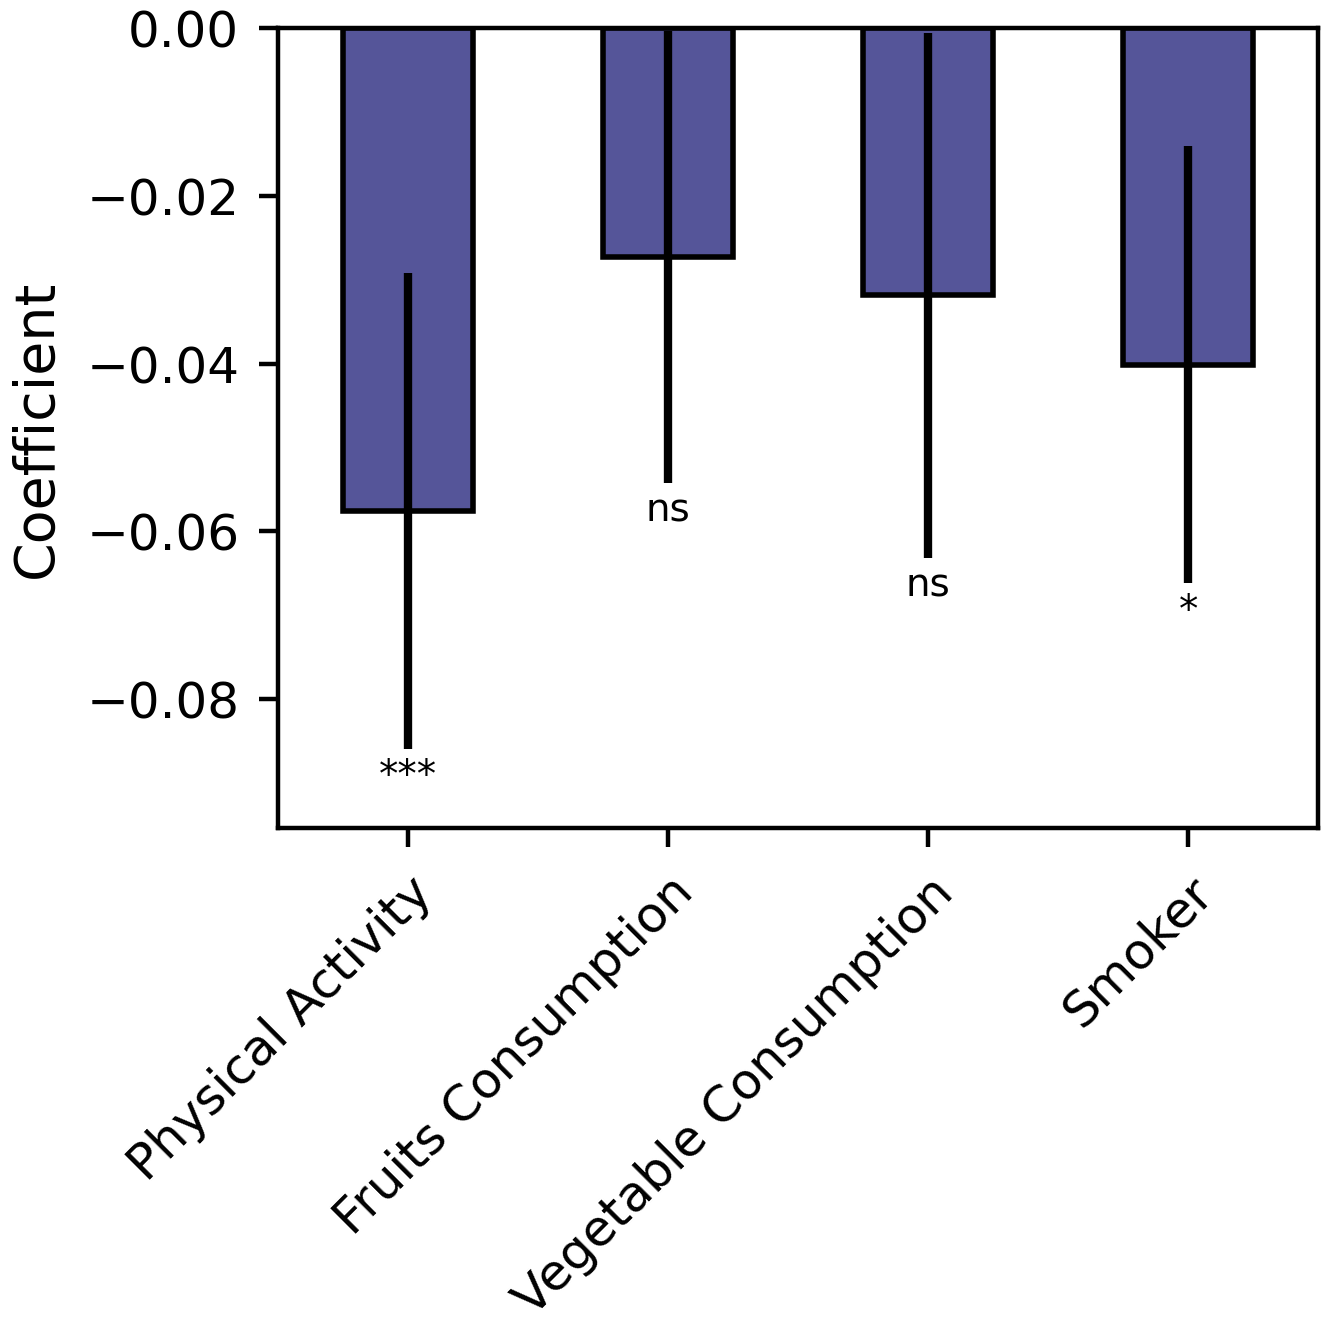
\includegraphics{df_lifestyle_combined_formatted.png}
\caption{Combined effects of lifestyle factors (physical activity, fruit and vegetable consumption, and smoking) on Diabetes
Smoker: 1: Yes, 0: No - Smoking status. 
Physical Activity: 1: Yes, 0: No - Engaged in physical activity in the past 30 days. 
Fruits Consumption: 1: Yes, 0: No - Consumed one or more fruits each day. 
Vegetable Consumption: 1: Yes, 0: No - Consumed one or more vegetables each day. 
CI: 95\% Confidence Interval. 
P-value: P-values indicating the significance of the coefficient. 
Significance: ns p $>$= 0.01, * p $<$ 0.01, ** p $<$ 0.001, *** p $<$ 0.0001.}
\label{figure:df-lifestyle-combined-formatted}
\end{figure}
% This latex figure presents "df_lifestyle_combined_formatted.png",
% which was created from the df:
% 
% index,"coef","CI","P-value"
% "Physical Activity",(*@\raisebox{2ex}{\hypertarget{C0a}{}}@*)-0.05757,((*@\raisebox{2ex}{\hypertarget{C0b}{}}@*)-0.08596, (*@\raisebox{2ex}{\hypertarget{C0c}{}}@*)-0.02919),(*@\raisebox{2ex}{\hypertarget{C0d}{}}@*)7.03e-05
% "Fruits Consumption",(*@\raisebox{2ex}{\hypertarget{C1a}{}}@*)-0.02723,((*@\raisebox{2ex}{\hypertarget{C1b}{}}@*)-0.05416, (*@\raisebox{2ex}{\hypertarget{C1c}{}}@*)-0.0002964),(*@\raisebox{2ex}{\hypertarget{C1d}{}}@*)0.0475
% "Vegetable Consumption",(*@\raisebox{2ex}{\hypertarget{C2a}{}}@*)-0.03183,((*@\raisebox{2ex}{\hypertarget{C2b}{}}@*)-0.06311, (*@\raisebox{2ex}{\hypertarget{C2c}{}}@*)-0.0005435),(*@\raisebox{2ex}{\hypertarget{C2d}{}}@*)0.0462
% "Smoker",(*@\raisebox{2ex}{\hypertarget{C3a}{}}@*)-0.04009,((*@\raisebox{2ex}{\hypertarget{C3b}{}}@*)-0.06621, (*@\raisebox{2ex}{\hypertarget{C3c}{}}@*)-0.01398),(*@\raisebox{2ex}{\hypertarget{C3d}{}}@*)0.00262
% 
% To create the figure, this df was plotted with the command:
% 
% df.plot(kind='bar', y=['coef'], ylabel='Coefficient')
% 
% Confidence intervals for y-values were then plotted based on column: ['CI'].
% 
% P-values for y-values were taken from column: ['P-value'].
% 
% These p-values were presented above the data points as stars (with significance threshold values indicated in the figure caption).
\end{codeoutput}
\hypertarget{file-df-log-reg-formatted-pkl}{}

\subsubsection*{\hyperlink{file-df-log-reg-pkl}{df\_log\_reg\_formatted.pkl}}

\begin{codeoutput}
\begin{table}[h]
\caption{Logistic regression results for the association between lifestyle factors and Diabetes, adjusted for confounders}
\label{table:df-log-reg-formatted}
\begin{threeparttable}
\renewcommand{\TPTminimum}{\linewidth}
\makebox[\linewidth]{%
\begin{tabular}{lrrrlrr}
\toprule
 & Coef. & Std.Err. & z & P$>$\textbar{}z\textbar{} & [0.025 & 0.975] \\
\midrule
\textbf{Physical Activity} & -0.04278 & 0.05044 & -0.8482 & 0.396 & -0.1416 & 0.05607 \\
\textbf{Fruits Consumption} & 0.1614 & 0.06097 & 2.648 & 0.0081 & 0.04194 & 0.2809 \\
\textbf{PA*Fruit} & -0.1368 & 0.07954 & -1.719 & 0.0855 & -0.2927 & 0.01913 \\
\textbf{Vegetable Consumption} & 0.02542 & 0.04913 & 0.5173 & 0.605 & -0.07087 & 0.1217 \\
\textbf{PA*Veggie} & 0.01096 & 0.06389 & 0.1715 & 0.864 & -0.1143 & 0.1362 \\
\textbf{Fruit*Veggie} & -0.2172 & 0.07334 & -2.962 & 0.00306 & -0.361 & -0.07349 \\
\textbf{PA*Fruit*Veggie} & 0.03538 & 0.09329 & 0.3793 & 0.704 & -0.1475 & 0.2182 \\
\textbf{Smoker} & -0.1666 & 0.04951 & -3.365 & 0.000766 & -0.2636 & -0.06955 \\
\textbf{PA*Smoker} & 0.07211 & 0.06833 & 1.055 & 0.291 & -0.06182 & 0.206 \\
\textbf{Fruit*Smoker} & 0.03003 & 0.08358 & 0.3593 & 0.719 & -0.1338 & 0.1938 \\
\textbf{PA*Fruit*Smoker} & 0.05552 & 0.1109 & 0.5007 & 0.617 & -0.1618 & 0.2728 \\
\textbf{Veggie*Smoker} & 0.03509 & 0.06504 & 0.5395 & 0.59 & -0.09239 & 0.1626 \\
\textbf{PA*Veggie*Smoker} & -0.01115 & 0.08623 & -0.1293 & 0.897 & -0.1802 & 0.1579 \\
\textbf{Fruit*Veggie*Smoker} & 0.06744 & 0.09989 & 0.6751 & 0.5 & -0.1283 & 0.2632 \\
\textbf{PA*Fruit*Veg*Smoker} & -0.05146 & 0.1292 & -0.3982 & 0.69 & -0.3047 & 0.2018 \\
\bottomrule
\end{tabular}}
\begin{tablenotes}
\footnotesize
\item Coef. = Coefficient; Std.Err. = Standard Error; P$>$\textbar{}z\textbar{} = P-value for Z-statistic. Interaction terms are denoted as PA (Physical Activity), Fruit (Fruits Consumption), Veggie (Vegetable Consumption), and Smoker.
\item \textbf{Smoker}: 1: Yes, 0: No - Smoking status
\item \textbf{Physical Activity}: 1: Yes, 0: No - Engaged in physical activity in the past 30 days
\item \textbf{Fruits Consumption}: 1: Yes, 0: No - Consumed one or more fruits each day
\item \textbf{Vegetable Consumption}: 1: Yes, 0: No - Consumed one or more vegetables each day
\item \textbf{PA*Fruit}: Interaction term between Physical Activity and Fruits Consumption
\item \textbf{PA*Veggie}: Interaction term between Physical Activity and Vegetable Consumption
\item \textbf{PA*Smoker}: Interaction term between Physical Activity and Smoking Status
\item \textbf{Fruit*Veggie}: Interaction term between Fruits and Vegetable Consumption
\item \textbf{Fruit*Smoker}: Interaction term between Fruits Consumption and Smoking Status
\item \textbf{Veggie*Smoker}: Interaction term between Vegetable Consumption and Smoking Status
\item \textbf{PA*Fruit*Veggie}: Three-way interaction term among Physical Activity, Fruits, and Vegetable Consumption
\item \textbf{PA*Fruit*Smoker}: Three-way interaction term among Physical Activity, Fruits Consumption and Smoking Status
\item \textbf{PA*Veggie*Smoker}: Three-way interaction term among Physical Activity, Vegetable Consumption and Smoking Status
\item \textbf{Fruit*Veggie*Smoker}: Three-way interaction term among Fruits, Vegetable Consumption and Smoking Status
\item \textbf{PA*Fruit*Veg*Smoker}: Four-way interaction term among Physical Activity, Fruits, Vegetable Consumption and Smoking Status
\item \textbf{z}: Z-statistic for the hypothesis test that the coefficient is zero
\end{tablenotes}
\end{threeparttable}
\end{table}

\end{codeoutput}

\end{document}
